\documentclass[TS]{sesamanuel}

% modifications dans la classe (fichier sesamanuel.cls) :
% 	voir manuel 6e

%%%%%%%
%Rajouté le 12/06/2018 SV et BN pour compilation espace insécable sous linux 
%\DeclareUnicodeCharacter{00A0}{~} %pour remplacer les espaces insécables
%\DeclareUnicodeCharacter{2011}{-}
%\usepackage{pdfpages}
%%%%%%%


% a priori, après l'impression du livre, tout ce fichier devrait être
% fusionné avec la classe principale, dernière version

\AtBeginDocument{\color{Noir}}

\renewcommand*\StringPrerequis{Connaissances
  n\'ecessaires \`a ce chapitre}

\usepackage{textcomp,pgfplots}
% standalone ne gère pas graphicspath... hum...
\newcommand{\standalonepath}[1]{#1}
% Au début de chaque chapitre on redéfinira cette commande en
% indiquant le chemin

\frenchbsetup{og=«,fg=»,}

\renewcommand\PrefixeCorrection{Corrections/}
\DeclareRemLike{intuition}{Idée intuitive}
\DeclareRemLike{exemples}{Exemples}


\newcommand*\StringExemples{Exemples}
\makeatletter
\newcommand*\smc@cartoucheexemples{% au pluriel
  \begin{pspicture}(-\ExempleVRuleWidthFrame,0)
                 (\ExempleWidthFrame,\ExempleHeightFrame)
    \psframe*[linewidth=0pt,linecolor=ExempleEdgeFrameColor]
             (-\ExempleVRuleWidthFrame,-\ExempleHRuleWidthFrame)
             (\ExempleWidthFrame,\ExempleHeightFrame)
    \psframe*[linewidth=0pt,linecolor=ExempleBkgFrameColor]
             (0mm,-0mm)(\ExempleWidthFrame,\ExempleHeightFrame)
    \rput[B](\dimexpr\ExempleWidthFrame/2,0){%
      \ExempleTitleFont
      \textcolor{ExempleTitleColor}{\StringExemples}%
    }
  \end{pspicture}%
}

\newenvironment{exemples*1}[1][]{%
  \par\addvspace{\BeforeExempleVSpace}
  \let\correction\smc@one@exemplecorrection
  \let\itemize\smc@exempleitemize
  \let\enditemize\endsmc@exempleitemize
  \let\colitemize\smc@exemplecolitemize
  \let\endcolitemize\endsmc@exemplecolitemize
  \let\enumerate\smc@exempleenumerate
  \let\endenumerate\endsmc@exempleenumerate
  \let\colenumerate\smc@exemplecolenumerate
  \let\endcolenumerate\endsmc@exemplecolenumerate
  \let\partie\smc@nopartie
  \let\exercice\smc@noexercice
  \let\endexercice\endsmc@noexercice
  \let\corrige\smc@nocorrige
  \let\endcorrige\endsmc@nocorrige
  \def\smc@currpart{Exemple}%
  \hspace*{\dimexpr \SquareWidth*3}%
  \color{ExempleRuleColor}%
  \vrule width \RuleWidth
  \hspace*{\dimexpr \SquareWidth-\RuleWidth}%
  \minipage[t]{\dimexpr\linewidth-\SquareWidth*4-\ExtraMarginRight}
    \smc@cartoucheexemples
    \space
    \color{Noir}%
    \ignorespaces
}
{%
  \endminipage
  \par
}

\DeclareRemLike{consequence}{Conséquence}
\DeclareRemLike{rappel}{Rappel}
\DeclareRemLike{valeurspart}{Valeurs particulières}
%\DeclareRemLike{theoreme}{Théorème}
% \NewThema{SP}
%          {sp}
%          {stat. et probabilités}
%          {Stat. et probabilités}
%          {STATISTIQUES\\ PROBABILITÉS}
%          {PartieStatistique}
%          {PartieStatistique}

\NewThema{A}
         {a}
         {analyse}
         {Analyse}
         {ANALYSE}
         {PartieFonction}
         {A3}


% Attention, il faudra ajouter un renewcommand \ListeMethodesThemes
% pour afficher la liste des méthodes à la fin du livre

% Si ils veulent changer la couleur du numéro des exos des
% auto-évaluations il faudra aller voir
% \colorlet{CorrigeNumExerciceFrameBkg}{J1}
 
\newcommand{\N}{\mathbb{N}} 
\newcommand{\R}{\mathbb{R}}
\newcommand{\Z}{\mathbb{Z}}
\renewcommand{\cfrac}[2]{{\displaystyle\frac{%
  \vrule height10pt depth0pt width0pt #1}{#2}}%
  \kern-\nulldelimiterspace}
%\usepackage{casio-fx,ti83symbols}

\newcommand\renvoimethode[1]{%
  Méthode \ref{#1}, p.~\pageref{#1}%
}

\newcommand*\calculatrice{%
  \psframebox[framesep=1pt,linewidth=\LogoLineWidth,
              linecolor=TiceLineColor, fillstyle=solid,
              fillcolor=TiceBkgColor, framearc=0.6]{%
    \TiceFont
    \textcolor{TiceTextColor}{CALC}%
  }
}
\newcommand\calc{\calculatrice}

% Chapitre G1 et G3
\newcommand{\covec}[2]{\left(\begin{array}{c} #1\\#2\end{array}\right)}

% Chapitre G2
\usepackage{tipa}
\newcommand{\arc}[1]{%
  \setbox9=\hbox{#1}%
  \ooalign{\resizebox{\wd9}{\height}{\texttoptiebar{\phantom{A}}}\cr#1}}

% Chapitre A4


\DeclareMathOperator{\e}{e}
\renewcommand{\cosh}{\operatorname{ch}}
\renewcommand{\sinh}{\operatorname{sh}}
\renewcommand{\tanh}{\operatorname{th}}

\newcommand*{\StringLEMM}{LEMME\footnote{Un \MotDefinition{lemme}{} est un résultat préliminaire ou  intermédiaire qui intervient parfois dans la preuve d'un théorème lorsqu'elle est un peu longue.}}
\newcommand*{\StringLEMME}{LEMME}
\DeclareDefLike{lemme}{\StringLEMME}
\DeclareDefLike{lemm}{\StringLEMM}

\newcommand*{\StringPROPRIETA}{PROPRIÉTÉ (admise)}
\DeclareDefLike{proprieta}{\StringPROPRIETA}

\usepackage{wrapfig}

% Environnement général pour toutes les fiches
\newcommand\AnnexeTICE{%
  \ChangeAnnexe{C2}{A1}{G1}{Blanc}%
  \annexe{}%
}
% Déclaration de l'environnement pour une fiche
\DeclareTPLike{ficheTICE}{Fiche}
              {TPTopColor}
              {TPBottomColor}
              {TPTitleColor} 
% Définition d'une commande \souspartie pour les besoins de la fiche
% TICE. C'est la commande \partie un peu revue. Je crée les mêmes
% paramètres de contrôle que pour TPPartie en mettant TPSousPartie à
% la place.

\colorlet{TPSousPartieColor}{J1}
\colorlet{TPSousPartieBkgColor}{C2}
\colorlet{TPSousPartieNumColor}{Blanc}
\newcommand*\TPSousPartieFont{\fontsize{10}{12}\sffamily\bfseries}
\def\BeforeTPSousPartieVSpace{3mm plus1mm minus1mm}
\def\AfterTPSousPartieVSpace{0mm plus1mm}
\edef\TPSousPartieHSep{\the\dimexpr\ItemRuleWidth+1.5mm}

\newcommand*\souspartie[1]{%
  \colorlet{smc@curr@partiecolor}{TPSousPartieNumColor}%
  \colorlet{smc@curr@partiebkgcolor}{TPSousPartieBkgColor}%
  \let\smc@curr@partiefont\TPSousPartieFont
  \par\addvspace{\BeforeTPSousPartieVSpace}
  \leavevmode
  \psframe*[linecolor=smc@curr@partiebkgcolor]
           (0,\ItemRuleDepth)(\ItemRuleWidth,\ItemRuleHeight)
  \hspace*{\TPSousPartieHSep}%
  \textcolor{TPSousPartieColor}{\TPSousPartieFont #1}
  \par\nobreak\addvspace{\AfterTPSousPartieVSpace}
}%

\newcommand\RoseItalTice[1]{\emph{\textcolor{C2}{#1}}}

%%% La présentation d'un texte en vis à vis d'une image n'est pas tout
%%% à fait un habillage et la répétition de tels éléments risque de
%%% poser des problèmes. Il vaut mieux se faire son propre « habillage
%%% »
\newcommand\ImageDroite[2]{%
  % #1 = texte
  % #2 = image (ou autre)
  \setbox4=\hbox{#2}%
  \dimen4=\dimexpr\ht4+\dp4-0.7\baselineskip
  \par
  \begin{tabularx}{\linewidth}{@{}Xc@{}}
    #1 & \raisebox{-\dimen4}{#2} %\box4
  \end{tabularx}
  \par
}
\newcommand{\commandetice}[1]{%
  \bgroup
  \shorthandoff{;:!?}%
  \texttt{#1}%
  \egroup
}

\newcommand\touchecalc[1]{%
  \tikz[baseline=-0.5ex]{\node at (0,0) [rounded corners = 2pt, draw, line width=.25pt]
    {\footnotesize\textsf{#1}}}%
}

\DeclareFontFamily{U}{tipa}{}
\DeclareFontShape{U}{tipa}{m}{n}{<->tipa10}{}
\newcommand{\arc@char}{{\usefont{U}{tipa}{m}{n}\symbol{62}}}%

\newcommand{\overarc}[1]{\mathpalette\arc@arc{#1}}

\newcommand{\arc@arc}[2]{%
  \sbox0{$\m@th#1#2$}%
  \vbox{
    \hbox{\resizebox{\wd0}{\height}{\arc@char}}
    \nointerlineskip
    \box0
  }%
}

% Pour A2

\def\psThomae{\pst@object{psThomae}}
\def\psThomae@i(#1,#2){%
   \begin@ClosedObj
   \addto@pscode{
     \psk@dotsize
     1 1 500 {
       dup
       /ipSave ED
       /ip ED
       1 1 500 {
         dup
         /iqSave ED
         /iq ED
         {
           iq 0 le { exit } if
           ip iq mod
           /ip iq def
           /iq ED
         } loop
         ip 1 eq {
           \psk@dotsize
           \@nameuse{psds@\psk@dotstyle}
           \pst@usecolor\pslinecolor ipSave iqSave div 1 iqSave div 
\tx@ScreenCoor
           2 copy moveto Dot
         } if
       } for
     } for
   }%
   \end@ClosedObj%
}

\renewcommand\smc@AfficheListeMethodesTheme[2]{%
  \expandafter\ifx\csname ifsmc@lom#1\endcsname\iftrue
    \csname smc@thema#2Color\endcsname
    \expandafter\smc@bandeaulistemethodes
      \expandafter{\csname StringListeMethode#2\endcsname}
    \ifnum \smc@NombreColonnesListeMethodes=\@ne
      \@starttoc{lom#1}
    \else
      \begin{multicols}{\smc@NombreColonnesListeMethodes}
        \@starttoc{lom#1}
      \end{multicols}
    \fi
  \fi
  \newpage
}
\fancypagestyle{empty}{%
  \fancyhead{}
  \fancyfoot{}
} 

\renewcommand*\AfficheCorriges[1][\NombreColonnesCorriges]{%
  \clearpage
  \label{toutes-solutions}
  \pagestyle{corrige}
  \thispagestyle{firstcorrige}
  \rput[Bl](0,9mm){\CorrigeTitleFont \MakeUppercase{\StringCorriges}}
  \vspace*{-5mm}
  \begingroup
  \columnsep \dimexpr \SquareWidth*2
  \columnseprule \CorrigeRuleWidth
  \def\columnseprulecolor{\color{ExerciceColumnRuleColor}}%
  \xdef\smc@NbColonneCorrige{#1}%
  \begin{multicols*}{#1}
  \raggedcolumns
    \@starttoc{cor}%
  \end{multicols*}
  \endgroup
}


\renewcommand\smc@preinsertlexiquefinal[3][]{%
  \@ifmtarg{#1}%
    {\smc@sansdiacritique{#2}}%
    {\smc@sansdiacritique{#1}}%
  \ifcsname affiche-\smc@tri\endcsname
  \else
    \expandafter\gdef\csname affiche-\smc@tri\endcsname{true}%
    \@ifmtarg{#1}%
      {\smc@sansdiacritique{#2}}%
      {\smc@sansdiacritique{#1}}%
    \global\advance\smc@numlexique \@ne
    \@ifmtarg{#1}%
      {\smc@@preFirstUppercase#2\@nil#3\@nil}%
      {\expandafter\protected@xdef\csname
lexique\the\smc@numlexique\endcsname
        {%
          \protect\textcolor{LexiqueEntreeColor}{%
            \protect\LexiqueEntreeFont #2%
          }%
%%%       \space\hbox to4.4em{\rdotfill}\kern0em\penalty0
          ~%%%
          \hspace*{\LexiquePageWidth}\penalty0
          \hspace{-\LexiquePageWidth}\dotfill
          \ifnum\csname nb-\smc@tri\endcsname>\@ne
            \protect\emph{ Pages~\csname pages-\smc@tri\endcsname}%
          \else
            \protect\emph{ Page~\csname pages-\smc@tri\endcsname}%
          \fi
        }%
      }%
    \expandafter\xdef\csname tri\the\smc@numlexique\endcsname
      {\smc@tri}%
  \fi
}
\long\def\smc@@preFirstUppercase#1#2#3\@nil#4\@nil{%
  \def\smc@arg{#1}%
  \ifx\smc@arg\smc@IeC
    \expandafter\protected@xdef\csname lexique\the\smc@numlexique\endcsname
      {%
        \protect\textcolor{LexiqueEntreeColor}
        {%
          \protect\LexiqueEntreeFont
          \MakeUppercase{#1#2}%
          \MakeLowercase{#3}%
        }%
        %%% \space\hbox to4.4em{\rdotfill}\kern-0.44em\penalty0
        ~%%%
        \hspace*{\LexiquePageWidth}\penalty0
        \hspace{-\LexiquePageWidth}\rdotfill
        \ifnum\csname nb-\smc@tri\endcsname>\@ne
          \protect\emph{ Pages~\csname pages-\smc@tri\endcsname}%
        \else
          \protect\emph{ Page~\csname pages-\smc@tri\endcsname}%
        \fi
      }%
  \else
    \expandafter\protected@xdef\csname lexique\the\smc@numlexique\endcsname
      {%
        \protect\textcolor{LexiqueEntreeColor}
        {%
          \protect\LexiqueEntreeFont
          \MakeUppercase{#1}%
          \MakeLowercase{#2#3}%
        }%
%%%     \space\hbox to4.4em{\rdotfill}\kern-0.44em\penalty0
        ~%%%
        \hspace*{\LexiquePageWidth}\penalty0
        \hspace{-\LexiquePageWidth}\rdotfill
        \ifnum\csname nb-\smc@tri\endcsname>\@ne
          \protect\emph{ Pages~\csname pages-\smc@tri\endcsname}%
        \else
          \protect\emph{ Page~\csname pages-\smc@tri\endcsname}%
        \fi
      }%
  \fi
} 

\makeatother

%\input{G1/biton} 

\usepackage{esvect,cancel} 
\newcommand{\chapeaumelon}[1]{\stackrel{\Large \frown}{#1}}

%%%%%%%% pour les figures en tikz
\usepackage{tikz,xparse}%xparse ajouté pour le compas en Tikz
\usepackage{tkz-tab,tkz-euclide}
\usetkzobj{all}
\usepackage{pgf}
\usetikzlibrary{arrows}
\usetikzlibrary{patterns}  
\definecolor{CyanTikz40}{cmyk}{.4,0,0,0}
\definecolor{CyanTikz20}{cmyk}{.2,0,0,0}

\definecolor{B1prime}      {cmyk}{0.00, 1.00, 0.00, 0.50}
\definecolor{H1prime}      {cmyk}{0.50, 0.00, 1.00, 0.00}

\tikzstyle{general}         =[font=\fontsize{7.5}{9}\selectfont,line width=0.3mm, >=stealth, x=1cm, y=1cm,line cap=round, line join=round]
\tikzstyle{quadrillage}     =[line width=0.3mm, color=CyanTikz40]
\tikzstyle{quadrillageNIV2} =[line width=0.3mm, color=CyanTikz20]
\tikzstyle{quadrillage55}   =[line width=0.3mm, color=CyanTikz40, xstep=0.5, ystep=0.5]
\tikzstyle{cote}            =[line width=0.3mm, <->]
\tikzstyle{epais}           =[line width=0.5mm, line cap=butt]
\tikzstyle{tres epais}      =[line width=0.8mm, line cap=butt]
\tikzstyle{axe}             =[line width=0.3mm, ->, color=Noir, line cap=rect]
\newcommand{\quadrillageSeyes}[2]{%
  \draw[line width=0.3mm, color=A1!10, ystep=0.2, xstep=0.8] #1 grid #2;
  \draw[line width=0.3mm, color=A1!30, xstep=0.8, ystep=0.8] #1 grid #2;
}

% ajouter pour manuel Flo
\newcommand*\circled[1]{\tikz[baseline=(char.base)]{
	\node[shape=circle,draw,inner sep=1pt] (char) {#1};}}

\newcommand{\axeX}[4][0]{%
  \draw[axe] (#2,#1)--(#3,#1);
  \foreach \x in {#4} {\draw (\x,#1) node {\small $+$};
    \draw (\x,#1) node[below] {\small $\numprint{\x}$};
  }%
}
\newcommand{\axeY}[4][0]{%
  \draw[axe] (#1,#2)--(#1,#3);
  \foreach \y in {#4} {\draw (#1, \y) node {\small $+$};
    \draw (#1, \y) node[left] {\small $\numprint{\y}$};
  }%
}
\newcommand{\axeOI}[3][0]{%
  \draw[axe] (#2,#1)--(#3,#1);
  \draw (1,#1) node {\small $+$};
  \draw (1,#1) node[below] {\small $I$};
}
\newcommand{\axeOJ}[3][0]{%
  \draw[axe] (#1,#2)--(#1,#3);
  \draw (#1, 1) node {\small $+$};
  \draw (#1, 1) node[left] {\small $J$};
}
\newcommand{\axeXgraduation}[2][0]{%
  \foreach \x in {#2} {\draw (\x,#1) node {\small $+$};}%
}
\newcommand{\axeYgraduation}[2][0]{%
  \foreach \y in {#2} {\draw (#1, \y) node {\small $+$};}%
}
\newcommand{\origine}{%
  \draw (0,0) node[below left] {\small $0$};
}
\newcommand{\origineO}{%
  \draw (0,0) node[below left] {$O$};
}
\newcommand{\point}[4]{%
  \draw (#1,#2) node[#4] {$#3$};
}
\newcommand{\pointGraphique}[4]{%
  \draw (#1,#2) node[#4] {$#3$};
  \draw (#1,#2) node {$+$};
}
\newcommand{\pointFigure}[4]{
  \draw (#1,#2) node[#4] {$#3$};
  \draw (#1,#2) node {$\times$};
}
\newcommand{\pointC}[3]{
  \draw (#1) node[#3] {$#2$};
}
\newcommand{\pointCGraphique}[3]{
  \draw (#1) node[#3] {$#2$};
  \draw (#1) node {$+$};
}
\newcommand{\pointCFigure}[3]{
  \draw (#1) node[#3] {$#2$};
  \draw (#1) node {$\times$};
}



\graphicspath{%
  {SimpMulDivFrac/Figures/}%
  {OpNombresDecimaux/Figures/}%
  {Angles/Figures/}%
  {Images/}%
}


% création d'un nouveau thème "calcul" pour le document
\NewThema{C}{c}{calcul}{Calcul}{CALCUL}{PartieFonction}{A3}

\renewcommand\ListeMethodesThemes{{c}{C},{g}{G}}
\renewcommand*\StringListeMethode{M\'ethodes du livret 1}

% création d'un nouveau thème "Manuel" pour le sommaire
%\NewThema{M}{m}{manuel}{Manuel}{MANUEL}{PartieFonction}{A3}

\usepackage{tikzpeople}
\usetikzlibrary{shapes.callouts}

\begin{document}



\begin{prerequis}[Un manuel de l'association Sésamath]
\begin{itemize}
\item  Ce manuel est adapté en partie du manuel Sésamath de l'association Sésamath:\\
\texttt{http://manuel.sesamath.net/}
\item … Et de l'association Sésamath Suisse romande:\\ \texttt{http://www.sesamath.ch/}
\item L'Institut Florimont a réalisé la transcription dans le langage de description de documents libre et gratuit \LaTeX{} en utilisant la classe \texttt{sesamanuel} développée par l'association Sésamath;
\item E. Villié a réalisé la couverture pour l'Institut Florimont;
\item Version Septembre 2019 --- Institut Florimont (Genève);\vspace{.3em}
\item Publication sous licence libre \hspace{1em} \raisebox{-0.4\height}{
\includegraphics[width=2cm]{cc-by-sa}}
\end{itemize}
 \end{prerequis}

\vspace{1em}
%%%%%%%%%%%%%%%%%%%%%%%%%%
%Fin page Sesamath
%%%%%%%%%%%%%%%%%%%%%%%%%%

%%%%%%%%%%%%%%%%%%%%%%%%%%
%%%%%%%%%%%%%%%%%%%%%%%%%%
%Pour finir
\colorlet{ChapterNumColor}{white}
\setcounter{chapter}{0}

%%%%%%%%%%%%%%%%%%%%%%%%%%%
%Fin Pour Finir…

\setcounter{page}{4}


%%%%%%%%%%%%%%%%%%%%%%%%%%%%%%
% Début des chapitres
%%%%%%%%%%%%%%%%%%%%%%%%%%%%%%

\themaC
\chapter{Opérations sur les nombres décimaux}\label{ChOpNombresDecimaux}

\vspace{5cm}
\begin{acquis}
\begin{itemize}
\item Savoir effectuer une succession d'opérations avec ou sans parenthèses, en respectant les règles de priorité et sans calculatrice.
\item Savoir donner une valeur approchée d'un nombre relatif (par excès, par défaut et troncature).
\columnbreak
\item Savoir résoudre des problèmes utilisant les 4 opérations, en n'utilisant qu'une seule expression mathématique.
\end{itemize}
\end{acquis}


%\activites  % pas d'activité dans ce chapitre
%\input{OpNombresDecimaux/OpNbDec_acti.tex}

\cours
\section{Rappels sur les opérations avec des nombres relatifs}

\subsection{Addition / soustraction de nombres relatifs}

\begin{rappel}
La \MotDefinition{valeur absolue}{} d'un nombre relatif est \textbf{le nombre sans son signe}. Sur une droite graduée, cela correspond à la distance entre l'origine et le point qui a pour abscisse ce nombre.
\end{rappel}


\begin{aconnaitre}
Pour \textbf{additionner deux nombres relatifs de même signe}, on additionne leur valeur absolue et on garde le signe commun.

Pour \textbf{additionner deux nombres relatifs de signes contraires}, on soustrait la plus petite valeur absolue de la plus grande et on prend le signe de celui qui a la plus grande valeur absolue.

\textbf{Soustraire un nombre relatif} revient à ajouter \textbf{son opposé} (\textbf{L'opposé d'un nombre relatif} est le nombre de signe contraire qui a la même valeur absolue).
\end{aconnaitre}


\begin{exemple*1}
Effectue l'addition suivante : $A = (-2) +(-3)$. 

\correction

\begin{tabular}{lcl}
$A = (-2) +(-3)$ & $\rightarrow$ & On veut additionner deux nombres relatifs de même signe. \\
$A = -(2 +3)$ & $\rightarrow$ & On additionne leur valeur absolue et on garde le signe commun : $-$. \\
$A = -5 $ & $\rightarrow$ &  On calcule. \\
\end{tabular}

\end{exemple*1}





\begin{exemple*1}
Effectue l'addition suivante : $B = (-5) +(+7)$.  

\correction

\begin{tabular}{lcl}
$B = (-5) +(+7)$ & $\rightarrow$ & On veut additionner deux nombres relatifs de signes contraires. \\
$B = +(7 -5)$ & $\rightarrow$ & On soustrait leur valeur absolue et on écrit le signe du nombre qui a \\
& & la plus grande valeur absolue $(+7)$. \\
$B = +2$ & $\rightarrow$ & On calcule. \\
\end{tabular}

\end{exemple*1}





\begin{exemple*1}
Effectue la soustraction suivante : $C = (-2) -(-3)$. 

\correction

\begin{tabular}{lcl}
$C = (-2) -(-3)$ & $\rightarrow$ &  On veut soustraire le nombre $-3$\\
$C = (-2) +(+3)$ & $\rightarrow$ &  On ajoute l'opposé de $-3$ qui est $+3$.\\
$C = +(3 -2)$ & $\rightarrow$ &  On ajoute deux nombres de signes contraires donc on soustrait \\
& & leur valeur absolue et on prend le signe du nombre qui a la plus \\
& & grande valeur absolue $(+3)$. \\
$C = +1$ & $\rightarrow$ &  On calcule.\\
\end{tabular}

\end{exemple*1}
 



\subsection{Multiplication / division de deux nombres relatifs}

\begin{aconnaitre}
Pour multiplier (ou diviser) deux nombres relatifs, on multiplie (ou on divise) leur valeur absolue et on applique la \MotDefinition{règle des signes}{} suivante :
\begin{itemize}
    \item le produit de deux nombres relatifs de \textbf{même signe} est \textbf{positif} ($"+" \times "+" = "+"$ et $"-" \times "-" = "+"$) ;
    \item le produit de deux nombres relatifs de \textbf{signes contraires} est \textbf{négatif} ($"+" \times "-" = "-"$ et $"-" \times "+" = "-"$).
\end{itemize}
\end{aconnaitre}	





\begin{exemple*1}
Effectue la multiplication : $F = (-4) \times (-2,5)$.

\correction
Le résultat est positif car c'est le produit de deux nombres relatifs de même signe (négatifs).

$F = 4 \times 2,5 \qquad F = 10$
\end{exemple*1}

\begin{exemple*1}
Effectue la division : $G = 6,8 \div (-2)$.

\correction
Le résultat est négatif car c'est le quotient de deux nombres de signes contraires (un nombre positif par un nombre négatif).

$G = -(6,8 \div 2) \qquad		G = -3,4$
\end{exemple*1}

\begin{remarque}
Multiplier un nombre relatif par $-1$ revient à prendre son opposé.
\end{remarque}


\subsection{Multiplication de plusieurs nombres relatifs}

\begin{aconnaitre}
Le produit de plusieurs nombres relatifs est : 
\begin{itemize}
    \item \textbf{positif} s'il comporte un nombre \textbf{pair} de \textbf{facteurs négatifs};
    \item \textbf{négatif} s'il comporte un nombre \textbf{impair} de \textbf{facteurs négatifs}.
\end{itemize}
\end{aconnaitre}

\begin{exemple*1}
Quel est le signe du produit : $H = -6 \times 7 \times (-8) \times (-9)$ ?

\correction
Le produit comporte trois facteurs négatifs. Or 3 est impair donc $H$ est négatif.
\end{exemple*1}


\begin{exemple*1}
Calcule le produit : $J = 2 \times (-4) \times (-5) \times (-2,5) \times (-0,8)$.

\correction
Le produit comporte quatre facteurs négatifs. Or 4 est pair donc $J$ est positif.
$J = 2 \times 4 \times 5 \times 2,5 \times 0,8$

$J = (2 \times 5) \times (4 \times 2,5) \times 0,8$

$J = 10 \times 10 \times 0,8 = 80 $
\end{exemple*1}


\section{Priorité des opérations}

\begin{aconnaitre}
Dans une suite d'opérations avec des nombres relatifs, on effectue \textbf{dans l'ordre} : d'abord les calculs entre parenthèses puis les calculs de puissances, les multiplications et divisions et enfin les additions et soustractions.
\end{aconnaitre}


\begin{exemple*1}
Effectue le calcul suivant : $M = -4 -5 \times (-2 -6)$.

\correction

\begin{tabular}{lcl}
$M = -4 -5 \times \underline{(-2 -6)}$ & $\rightarrow$ & On repère le calcul prioritaire. \\
$M = -4 \underline{-5 \times (-8)}$ & $\rightarrow$ & On effectue d'abord le calcul entre parenthèses. \\
$M = \underline{-4 + 40}$ & $\rightarrow$ & On effectue ensuite la multiplication. \\
$M = 36$ & $\rightarrow$ & On termine par l'addition. \\
\end{tabular}
\end{exemple*1}





\section{Approximation de nombres relatifs}

\subsection{Troncature}

\begin{definition}
Prendre la troncature d’un nombre à une précision donnée, c’est couper ce nombre et enlever tous les chiffres qui dépassent la précision demandée.
\end{definition}

\begin{exemple*1}
Donner la troncature à $10^{-2}$ de $349,7275$ et la troncature au dixième de $57,93$.
\correction
La troncature à $10^{-2}$ de $349,7275$ est $349,72$ et la troncature au dixième de $57,93$ est $57,9$.
\end{exemple*1}

\subsection{Valeur approchée par défaut et par excès}
 
\begin{remarque}
Lorsqu’un nombre comporte plusieurs chiffres après la virgule, on peut en donner une valeur approchée à :
$10^{-1}$ près, c’est-à-dire 1 chiffre après la virgule. C’est une valeur approchée au dixième.
$10^{-2}$ près, c’est-à-dire 2 chiffres après la virgule. C’est une valeur approchée au centième.
$10^{-3}$ près, c’est-à-dire 3 chiffres après la virgule. C’est une valeur approchée au millième.
\end{remarque}

\begin{definition}
La \MotDefinition{valeur approchée à l’unité par défaut}{} d’un nombre est le nombre entier immédiatement plus petit que notre nombre.

La \MotDefinition{valeur approchée à l’unité par excès}{} d’un nombre est le nombre entier immédiatement plus grand que notre nombre.
\end{definition}

\begin{exemple*1}
Donner les valeurs approchées par défaut et par excès, à l'unité, du nombre $12,58$.

\correction
Le nombre entier immédiatement plus petit que $12,58$ est $12$. Donc la valeur approchée par défaut à l'unité de $12,58$ est $12$. Le nombre entier immédiatement plus grand que $12,58$ est $13$. Donc la valeur approchée par excès à l'unité de $12,58$ est $13$.
\end{exemple*1}



\begin{definition}
La \MotDefinition{valeur approchée au dixième par défaut}{} d’un nombre est le nombre décimal ayant un seul chiffre après la virgule immédiatement plus petit que notre nombre.

La \textbf{valeur approchée au dixième par excès}{} d’un nombre est le nombre décimal ayant un seul chiffre après la virgule immédiatement plus grand que notre nombre.
\end{definition}

\begin{exemple*1}
Donner les valeurs approchées par défaut et par excès au dixième du nombre $8,193$.

\correction
Le nombre ayant un chiffre après la virgule et qui est immédiatement plus petit que $8,193$ est $8,1$. Donc la valeur approchée par défaut au dixième (ou à $10^{-1}$) de $8,193$ est $8,1$. Le nombre ayant un chiffre après la virgule et qui est immédiatement plus grand que $8,193$ est $8,2$. Donc la valeur approchée par excès au dixième (ou à $10^{-1}$) de $8,193$ est $8,2$.
\end{exemple*1}


\begin{remarque}
On définit de la même façon la valeur approchée par défaut ou par excès à une précision donnée : valeur approchée par défaut à 10-2 près (au centième), ou valeur approchée par excès à 10-4 près (au dix-millièmes) ...
\end{remarque}


\subsection{Arrondi}

\begin{definition}
Donner l’arrondi d’un nombre positif, c’est déterminer \textbf{une valeur approchée de ce nombre en fonction du chiffre qui suit directement sa troncature} :
\begin{itemize}
    \item Si ce chiffre est 0, 1, 2, 3 ou 4, l’arrondi correspond à la troncature.
    \item Si ce chiffre est 5, 6, 7, 8 ou 9, on rajoute 1 au dernier chiffre de sa troncature.
\end{itemize}
\end{definition}

\begin{exemple*1}
Donner les arrondis à $10^{-2}$ et $10^{-3}$ de $83,372851$. Donner la troncature au dixième et l’arrondi au dixième de $175,378$.
\correction
L'arrondi à $10^{-2}$ de $83,374851$ est $83,37$ (car le chiffre des millièmes est 4) et l'arrondi à $10^{-3}$ est $83,375$ (car le chiffre des dix-millièmes est 8).

La troncature au dixième de $175,378$ est $175,3$ et l’arrondi au dixième est $175,4$ (car le chiffre des centièmes est 7).
\end{exemple*1}


\exercicesbase
\begin{colonne*exercice}

\serie{Additionner et soustraire}


\begin{exercice}Effectue les additions suivantes :
\begin{enumerate}
\item $(+4) +(+9)$
\item $(-2) +(+3)$
\item $(-4) +(-11)$
\item $(+1) +(-7)$
\item $(-10) +(+10)$
\item $(-40) +(+20)$
\end{enumerate}
\end{exercice}


\begin{exercice}Effectue les calculs suivants :
\begin{enumerate}
\item $9 -12$
\item $-10 -6$
\item $-2 - (-17)$
\item $-13 - (-5)$
\item $8 -1$
\item $0 -(-72)$
\end{enumerate}
\end{exercice}


\begin{exercice}Effectue les calculs suivants :
\begin{enumerate}
\item $15,7 +22,8$
\item $-51,5 +31,7$
\item $7,2 -3,1$
\item $31,2 -13,4$
\item $-2,8	- (-3,9)$
\item $-50	-12,4$
\end{enumerate}
\end{exercice}


\begin{exercice}Effectue les calculs suivants :
\begin{enumerate}
\item $5 -17$
\item $8 -21$
\item $-5 -2$
\item $-7 +11$
\item $31 -37$
\item $-2,8 -2,1$
\item $-8,3 +3,5$
\item $1,7 -3,52$
\end{enumerate}
\end{exercice}


\begin{exercice}Effectue les calculs suivants :
\begin{enumerate}
\item $13,2 +12,8$
\item $-25,5 +11,7$
\item $2,3 +(-1,5)$
\item $17,4 - (12,6)$
\item $-3,9 - (-11,1)$
\item $-100 - (+13)$
\end{enumerate}
\end{exercice}



\begin{exercice}Effectue les calculs suivants (tu peux  regrouper les termes de même signe) :

$A = 24 +8 -12 +1 -5$

$B = -14 +5 -7 -10 +13$

$C = 11 -(-5) +(-8) +1 -(+17)$

$D = -11 -(+4) +23 +(-12) -(-18)$
\end{exercice}



\begin{exercice}Effectue les calculs suivants (tu peux  regrouper les termes de même signe) :

$A = 15 +3 -6 +2 -7 $

$B = -8 +4 -5 -6 +11$

$C = 10 -(-4) +(-1) +5 -9$

$D = (-15) -(+14) +30 +(-15) -(-20)$
\end{exercice}


\begin{exercice}Regroupe les termes astucieusement puis calcule :

$A = 22 +25 +8 -25$

$B = -1,5 +5,7 -3,6 +0,3 +1,5$
\end{exercice} 



\serie{Multiplier}



\begin{exercice}Calcule mentalement :
\begin{enumerate} 
\item $(-8) \times (+2)$
\item $(-2) \times (+5)$
\item $(-4) \times (-8)$
\item $(+9) \times (+10)$
\item $(+191) \times (+0,1)$ 
\item $(-1,5) \times (+20)$
\item $(-0,25) \times (-4)$
\item $(+0,8) \times (-3)$
\item $(-3,2) \times (+4)$
\item $(-1) \times (-17)$
\end{enumerate}
\end{exercice}



\begin{exercice}Relie chaque calcul à son résultat :
\begin{colitemize}{2}
\item $(+5) \times (-7)$
\item $(-6) \times (-4)$
\item $(-4) \times (+3)$
\item $(+7)	\times (+7)$
\item $(-3) \times (-4)$
\item $(-9) \times (-3)$
\item $(-5) \times (+3)$
\item $(-8) \times (+6)$
\item $-15$
\item $-35$
\item $-12$
\item $+12$
\item $-48$
\item $+27$
\item $+24$
\item $+49$
\end{colitemize}
\end{exercice}



\begin{exercice}Calcule, sachant que $11,2 \times 2,5 = 28$ :
\begin{enumerate}
\item $11,2 \times (-2,5)$
\item $-11,2 \times (-2,5)$
\end{enumerate}
\end{exercice}



\begin{exercice}[Un produit peut en cacher un autre...]
\begin{enumerate}
\item Calcule le produit $7,5 \times 0,2$.
\item Effectue alors les calculs suivants :
\subitem $A = 7,5 \times (-0,2)$
\subitem $B = (-0,2) \times (-7,5)$
\subitem $C = (-75) \times (+0,2)$
\subitem $D = (-7,5) \times (-20)$
\end{enumerate}
\end{exercice}



\begin{exercice}Complète les « pyramides » suivantes sachant que le nombre contenu dans une case est le produit des nombres contenus dans les deux cases situées en dessous de lui :
\end{exercice}


\begin{exercice}Effectue les calculs suivants :

$A = (-4) \times (-7) \times (+5)$

$B = (-2) \times (-5) \times (-3)$

$C = (+5) \times (-1) \times (+9)$
\end{exercice}



\begin{exercice}Effectue les calculs suivants :

$A = (-2,2) \times (-10) \times (+3) \times (-0,5)$

$B = (-50) \times (-0,25) \times (+4) \times (+2)$

$C = (-4) \times (-0,1) \times (+5) \times (+4)$

$D = (-1,5) \times (+4) \times (-1) \times (+0,8) \times (-3)$

$E = (+4) \times (-10) \times (+2) \times (-1) \times (-1)$
\end{exercice}



\begin{exercice}Calcule astucieusement :

$A = (-2) \times (-1,25) \times (-2,5) \times (-8)$

$B = (-75) \times (-0,25) \times (+2) \times (+4)$

$C = (+0,01) \times (-25) \times (-13) \times 4 \times (-3)$
\end{exercice}



\begin{exercice}Calcule dans chaque cas le produit $xy$ :
\begin{enumerate}
\item $x = 5 et y = -3$
\item $x = +4 et y = -11$
\item $x = -2 et y = -5$
\item $x = -0,5 et y = -5,2$
\end{enumerate}
\end{exercice}



\begin{exercice}Complète le tableau suivant :

\renewcommand*\tabularxcolumn[1]{>{\centering\arraybackslash}m{#1}}
\renewcommand{\arraystretch}{1.6}
\begin{ltableau}{\linewidth}{6}
\hline
$a$ & $b$ & $c$ & $ab$ &  $-(ac)$ & $abc$ \\ \hline 
$-5$ & 6 & $-4$ & & &  \\ \hline
$-1$ & $-2$ & $-3$ &  & & \\ \hline
$-2,1$ & $-4$ & $+3$  & & & \\ \hline
\end{ltableau}
\end{exercice}



\begin{exercice}[Décompositions...]
\begin{enumerate}
\item Trouve toutes les façons de décomposer le nombre $-20$ en produit de deux nombres entiers relatifs.
\item Trouve toutes les façons de décomposer le nombre 24 en produit de trois nombres entiers relatifs.
\end{enumerate}
\end{exercice} 



\serie{Diviser}



\begin{exercice}Calcule mentalement :
\begin{enumerate}
\item $64 \div (-4)$
\item $48 \div (-8)$
\item $-27 \div (-3)$
\item $72 \div (+9)$
\item $-71 \div ( -1)$
\item $-42 \div 7$
\item $(-42) \div (-6)$
\item $125 \div (-5)$
\item $(-7) \div (+7)$
\item $(-29) \div (+1)$
\end{enumerate}
\end{exercice}



\begin{exercice}Calcule mentalement :
\begin{enumerate}
\item $(-100) \div (+25)$
\item $(-42) \div (-4)$
\item $(+54) \div (-3)$
\item $(+55) \div (+5)$
\item $(-24) \div (-5)$
\item $(-13) \div (-10)$
\end{enumerate}
\end{exercice}


\begin{exercice}Pour chaque fraction, trouve l'écriture la plus simple possible : 

Exemple : $\dfrac{-2}{+9}=-\dfrac{2}{9}$
\begin{enumerate}
\item $-\dfrac{+4}{+5}$
\item $-\dfrac{-1}{-5}$
\item $\dfrac{7}{-3}$
\item $-\dfrac{-8}{11}$
\item $-\dfrac{1}{-10}$
\item $-\dfrac{5}{-15}$
\end{enumerate}
\end{exercice}



\begin{exercice}Sans calculatrice, donne l'écriture décimale de chacun des nombres suivants :
\begin{enumerate}
\item $-\dfrac{3}{-10}$
\item $-\dfrac{-64}{-8}$
\item $\dfrac{-50}{+100}$
\item $\dfrac{-3}{-2}$
\end{enumerate}
\end{exercice}



\begin{exercice}Utilise ta calculatrice pour donner l'écriture décimale des nombres suivants :
\begin{enumerate}
\item $\dfrac{-5}{-40}$
\item $-\dfrac{172}{-5}$
\item $-\dfrac{-125}{-625}$
\item $\dfrac{-0,235}{+0,8}$
\end{enumerate}
\end{exercice}



\begin{exercice}Dans chaque cas, calcule le quotient de $x$ par $y $:
\begin{enumerate}
\item $x = -15$ et $y = -3$
\item $x = +64$ et $y = -8$
\item $x = -36$ et $y = 12$
\item $x = -2,4$ et $y = 1,2$
\item $x = y = -2,3$
\item $x = 0$ et $y = -5$
\end{enumerate}
\end{exercice}



\begin{exercice}Complète le tableau suivant et donne le résultat sous forme décimale :

\renewcommand*\tabularxcolumn[1]{>{\centering\arraybackslash}m{#1}}
\renewcommand{\arraystretch}{1.6}
\begin{ltableau}{\linewidth}{6}
\hline
$a$ & $b$ & $c$ & $a \div b$ &  $-(b) \div c$ & $c \div (-a)$ \\ \hline 
$-5$ & 4 & $-4$ & & &  \\ \hline
$-2,5$ & $-1$ & $+20$ &  & & \\ \hline
$+8$ & $-4$ & $-0,5$  & & & \\ \hline
$-2,4$ & $-1,2$ & $-24$  & & & \\ \hline
\end{ltableau}
\end{exercice} 



\serie{Calculs variés}



\begin{exercice}Pour chacun des calculs suivants, indique s'il s'agit d'une somme ou d'un produit puis donne le résultat :
\begin{enumerate}
\item $-4 \times (+9)$
\item $-3 -(+8)$
\item $-7 +(-5)$
\item $+3 \times (-7)$
\item $-8 +(+6)$
\item $+9 \times (+3)$
\item $-5 -(-16)$
\item $-11 \times (-4)$
\end{enumerate}
\end{exercice}



\begin{exercice}Sans les calculer, donne le signe de chacun des calculs suivants :
\begin{enumerate}
\item $(-4) \times (-12)$
\item $(+15) +(-22)$
\item $(-45) -(-51)$
\item $(-37) \times (+51)$
\item $(+7) \times (+8)$
\item $(-7) +(+8)$
\item $(-3,12) \times (-2,5)$
\item $(-3,17) -(+3,7)$
\end{enumerate}
\end{exercice}



\begin{exercice}Calcule mentalement :
\begin{enumerate}
\item $8 \times (-8)$
\item $-22 +(-6)$
\item $-14 \times 3$
\item $-5 -(+17)$
\item $(-34) +(-19)$
\item $-15 \times (-5)$
\end{enumerate}
\end{exercice}



\begin{exercice}Calcule mentalement :
\begin{enumerate}
\item $(-4) \times (-2,5)$
\item $(+3,5) +(-2,2)$
\item $(-3,9) +(-5,4)$
\item $(-3) \times (+4,2)$
\item $(+3,4) \times (-2)$
\item $(-7,15) -(-2,2)$
\item $(-3,12) \times (-10)$
\item $(-0,7) -(+1,17)$
\end{enumerate}
\end{exercice}



\begin{exercice}Complète les « pyramides » suivantes sachant que le nombre contenu dans une case est le produit des nombres contenus dans les deux cases situées en dessous de lui :
\begin{center}
    \begin{tikzpicture}
    \node[name=a,businessman,minimum size=1.5cm] at (-2,0) {};
    \node[ellipse callout, draw,yshift= 1cm,xshift=.5cm, callout absolute pointer={(a.mouth)},    font=\footnotesize] {Deux pyramides ici !};

    \end{tikzpicture}
\end{center}
\end{exercice}



\begin{exercice}Effectue les calculs suivants en soulignant, à chaque étape, le calcul en cours :

$A = 7 +(-6) \times (-6)$

$B = 13 -(+3) \times (-4) -8$

$C = -30 \div (-9 +15)$

$D = -3 -9 \times (-3)$

$E = -3 \times 6 \times (-2 +8)$
\end{exercice}



\begin{exercice}Effectue les calculs suivants en soulignant, à chaque étape, le calcul en cours :

$A = -22 +(13 -5) \times (-5)$

$B = (-2) \times (-8) +2 \times (-20) \div 4$

$C = -28 +(5 -2) \times (-4)$

$D = 7 \times (-7) +3 \times (-25) \div (-5)$

$E = -3,1 \times (-6) +(-2,3 -7,7)$

$F = 150 \div (-3 -9 \times 3)$
\end{exercice}



\begin{exercice}Effectue les calculs suivants :

$A = 18 -[(-7 +13 ) -( 5 -23) -( 15 -8 )] -13$

$B = 28 \div (-3 \times 4 -2)$

$C = [13 -(-2)] \times 2 +5$

$D = (- 4 - 4 \times (- 4)) \div (2 \times (- 3))$

$E = [(-3) \times (-1 -4) +(-12) \div 4] \times (-3) +5$
\end{exercice}




\begin{exercice}Calcule les expressions suivantes :

$A = \dfrac{11}{2-5}$

$B = \dfrac{-6-3}{2+7}$

$C = \dfrac{-2-(-4)}{6-7}$
\end{exercice}



\begin{exercice}Effectue les calculs suivants :

$A = 16 \div (-2 \times 5 +2)$

$B = - 42 \div (-6 \times 3 +25)$

$C = [-8 -(-3)] \times 3 +4$

$D = (4 - 3 \times (- 4)) \div 4 -2$

$E = 62 \div 4 -(42 -2 \times 6) -7 +9 \times 2$
\end{exercice}




\begin{exercice}[Vocabulaire]
\begin{enumerate}
\item Traduis les phrases suivantes par un calcul :
    \begin{itemize}
    \item La somme du produit de 4 par $-5$ et de $-6$.
    \item Le produit de la somme de 7 et de $-8$ par la somme de 8 et de $-2$.
    \end{itemize}
\item Effectue ces calculs.
\end{enumerate}
\end{exercice}


\begin{exercice}[Vocabulaire (bis)]
\begin{enumerate}
\item Traduis les phrases suivantes par un calcul :
    \begin{itemize}
    \item La différence du quotient de 16 par $-2$ et de $-5$.
    \item Le quotient de la différence de 13 et de $-2$ par la somme de $-2$ et de $-3$.
    \end{itemize}
\item Effectue ces calculs.
\end{enumerate}
\end{exercice}



\begin{exercice}[Vocabulaire (ter)]
\begin{enumerate}
\item Traduis les phrases suivantes par un calcul :
    \begin{itemize}
    \item Le produit du quotient de 24 par $-4$ par la somme de 3 et de $-6$.
    \item La différence du quotient de $-63$ par 7 et de  la somme de $-4$ et de $-5$.
    \end{itemize}
\item Effectue ces calculs.
\end{enumerate}
\end{exercice}



\begin{exercice}[Vocabulaire (dans l'autre sens !)]

\begin{enumerate}
\item Traduis les expressions mathématiques suivantes par des phrases :

Exemple : $(-2) \times 3 +1$ se traduit par :
\og La somme du produit de $(-2)$ par 3 et de 1.\fg
    \begin{itemize}
    \item $A = 5 \times (-7) +3$
    \item $B = 3 + \dfrac{2}{-4}$
    \item $C = 7 - 4 \times (-10)$
    \item $D = (2 - 3) \times (-1 -2)$
    \item $E = \dfrac{1-7}{2+5}$
    \item $F = -2 +(-6) \times (-6) -9$
    \end{itemize}
\item Effectue ces calculs.
\end{enumerate}
\end{exercice}


\begin{exercice}Complète le tableau suivant :

\renewcommand*\tabularxcolumn[1]{>{\centering\arraybackslash}m{#1}}
\renewcommand{\arraystretch}{1.6}
\begin{ltableau}{\linewidth}{5}
\hline
$a$ & $b$ & $c$ & $ab-c$ &  $(a-b)c$ \\ \hline 
$2$ & 3 & $5$ & &  \\ \hline
$-1$ & $5$ & $6$  & & \\ \hline
$3$ & $-5$ & $-7$  & & \\ \hline
$-8$ & $2$ & $-6$  & & \\ \hline
\end{ltableau}
\end{exercice}



\begin{exercice}Pour $a = 3$, $b = -4$, $c = -5$ et $d = 7$, calcule les expressions suivantes :

$A = a -b +c$

$B = 2a -3b$

$C = ac -bd$

$D = -5ac +bd$

$E = 2(a  - b) +d$

$F = 5(b  -a) \div d$
\end{exercice}



\begin{exercice}Complète le tableau suivant :

\renewcommand*\tabularxcolumn[1]{>{\centering\arraybackslash}m{#1}}
\renewcommand{\arraystretch}{1.6}
\begin{ltableau}{\linewidth}{6}
\hline
$a$ & $b$ & $c$ & $ab$  & $(-ac)$ & $abc$ \\ \hline 
$-5$ &  & $+4$ & 10 & &  \\ \hline
 &  & $2$ & &  $-12$ & $-36$ \\ \hline
\end{ltableau}
\end{exercice}




\begin{exercice}Supprime les parenthèses dans chaque expression puis calcule sans calculatrice :

$A = [(-5) +6 - (-1) - 7] - [(-5) +6 - (-1) - 7]$

$B = [(-5) +6 - (-1) - 7] - [(-5) +6 - (-1) +7]$

$C = -18,1 +2,8 -7 +(-2,8 +18,1 -7)$

$D = 18,1 +2,8 -7 -(2,8 +18,1 +7)$
\end{exercice}



\begin{exercice}Effectue les calculs suivants en respectant les priorités :
\begin{enumerate}
\item $36 +(6 - 2)3 : 2 +102 - 4 +5 \times 2 - 1$
\item $(9 - 2)2 : 7 - 1 +43 : 16 - 5$
\item $92 : 3 +5 - (5 - 2) +36 +4$
\item $(12 - 2)2 : 20 +56 : 23 +25 - 5 : 5$
\item $25 +5 : 5 - 22 +6 +2 \times 3 - 1$
\item $451 - 12 \times 5 +60 \times 4$
\end{enumerate}
\end{exercice}



\begin{exercice}Effectue les calculs suivants en respectant les priorités :
\begin{enumerate}
\item $3^2 - 2^4 \times (9 - 10 +5) - 2 \times (5 +3^2)$
\item $2^4 : 4 - 2^3 \times 5^2 - 4^3 : 2^3 +36$
\item $10^2 - 4^2 \times (3^2 - 12 +2) +3$
\item $(3$$4 +2 - 3^0 +5^2) - 4 \times (- 3 +6^2 +1^4)$
\item $(3^2 - 2^3) \times 5 +2 \times (3 +1^5)$
\item $(3 \times 5 +2^2) \times 2 +(6 - 3 \times 2)^2$ 
\item $2 \times ( - 8) +8^2 $
\item $(350 : 10) \times (4^2 - 12)$
\end{enumerate}
\end{exercice}


\serie{Approximation}


\begin{exercice}On considère le nombre  $349,2856$.
\begin{enumerate}
\item Donner les troncatures : à l'unité, à $10^{-2}$ près, à $0,001$ près et à la centaine de ce nombre.
\item Donner les arrondis : à l'unité, au dixième, à $10^{-3}$ près, à la dizaine, à $0,01$ près de ce nombre.
\end{enumerate}
\end{exercice}



\begin{exercice}Recopier et compléter le tableau suivant :

\renewcommand*\tabularxcolumn[1]{>{\centering\arraybackslash}m{#1}}
\renewcommand{\arraystretch}{1.6}
\begin{cltableau}{\linewidth}{5}
\hline
nombre & valeur arrondie à l'unité & tron\-ca\-ture à $10^{-1}$ & valeur approchée à $10^{-2}$ par excès & valeur approchée à $10^{-1}$ par défaut \\ \hline
 $385,1829$ & & & & \\ \hline
 $17,4351$ & & & & \\ \hline
 $0,8796$ & & & & \\ \hline
\end{cltableau}
\end{exercice}




\begin{exercice}Complète les tableaux suivants avec les valeurs arrondies et les troncatures à l’unité, à $10^{-1}$ près, et au millième des nombres donnés.

\renewcommand*\tabularxcolumn[1]{>{\centering\arraybackslash}m{#1}}
\renewcommand{\arraystretch}{1.6}
\begin{cltableau}{\linewidth}{4}
\hline
nombre & valeur arrondie à l'unité & valeur arrondie à $10^{-1}$ & valeur arrondie au millième \\ \hline
$445,2541$ & & &  \\ \hline
$225,1247$ & & &  \\ \hline
$222,29143$ & & &  \\ \hline
$5,1452$ & & &  \\ \hline
$0,1726$ & & &  \\ \hline
$4,9273$ & & &  \\ \hline
$3,4216$ & & &  \\ \hline
$12,9214$ & & &  \\ \hline
\end{cltableau}

\vspace{1em}

\renewcommand*\tabularxcolumn[1]{>{\centering\arraybackslash}m{#1}}
\renewcommand{\arraystretch}{1.6}
\begin{cltableau}{\linewidth}{4}
\hline
nombre & tron\-ca\-ture à l'unité & tron\-ca\-ture à $10^{-1}$ & tron\-ca\-ture au millième \\ \hline
$445,2541$ & & &  \\ \hline
$225,1247$ & & &  \\ \hline
$222,29143$ & & &  \\ \hline
$5,1452$ & & &  \\ \hline
$0,1726$ & & &  \\ \hline
$4,9273$ & & &  \\ \hline
$3,4216$ & & &  \\ \hline
$12,9214$ & & &  \\ \hline
\end{cltableau}
\end{exercice}




\begin{exercice}Complète les tableaux suivants avec les valeurs approchées par excès et par défaut à l'unité, au dixième et au millième des nombres donnés.

\renewcommand*\tabularxcolumn[1]{>{\centering\arraybackslash}m{#1}}
\renewcommand{\arraystretch}{1.6}
\begin{cltableau}{\linewidth}{4}
\hline
nombre & valeur approchée par excès à l'unité & valeur approchée par défaut à l'unité & valeur approchée par excès à $10^{-1}$ \\ \hline
$23,1785$ & & &  \\ \hline
$193,3591$ & & &  \\ \hline
$18,5555$ & & &  \\ \hline
$0,0101$ & & &  \\ \hline
$385,854$ & & &  \\ \hline
$10,985$ & & &  \\ \hline
\end{cltableau}

\vspace{1em}

\renewcommand*\tabularxcolumn[1]{>{\centering\arraybackslash}m{#1}}
\renewcommand{\arraystretch}{1.6}
\begin{cltableau}{\linewidth}{4}
\hline
nombre & valeur approchée par défaut à $10^{-1}$ & valeur approchée par excès au millième & valeur approchée par défaut au millième \\ \hline
$23,1785$ & & &  \\ \hline
$193,3591$ & & &  \\ \hline
$18,5555$ & & &  \\ \hline
$0,0101$ & & &  \\ \hline
$385,854$ & & &  \\ \hline
$10,985$ & & &  \\ \hline
\end{cltableau}
\end{exercice}



\begin{exercice}Donne la troncature à $10^{-1}$, l'arrondi à 
$10^{-2}$ et la valeur approchée par excès à l'unité des nombres suivants :
\begin{enumerate}
\item $12,345$
\item $67,891$
\item $0,0001$
\item $958,12$
\item $25,0102$
\item $5,5$
\end{enumerate}
\end{exercice} 



\begin{exercice}Donne, à l'aide de ta calculatrice, l'arrondi à l'unité de chacun des nombres suivants, comme dans l'exemple :

Exemple : $A =\dfrac{-153}{23}$. La calculatrice donne $A \approx -6,652173913$. On a donc : $-7 < A < -6$. L'arrondi à l'unité de $A$ est $-7$ car $A$ est plus proche de $-7$ que de $-6$.

\vspace{.5em}

$B =\dfrac{39}{-9}$ 

$C = \dfrac{-17}{-7}$ 

$D = \dfrac{-28}{51}$ 
\end{exercice}

\end{colonne*exercice}


\exercicesappr
\begin{colonne*exercice}
\begin{exercice}
La différence de $a-b$ est égale à 12. On augmente $a$ de 3 et on diminue $b$ de 4. Combien vaut la différence entre ces deux nouveaux nombres ?
\end{exercice}


\begin{exercice}[Triangle magique]
La somme des nombres de chaque côté du triangle est 2. Remplis les cases vides avec les nombres relatifs $(-2)$ ; $(-1)$ ; 1 ; 2 et 3.
\begin{center}
    \begin{tikzpicture}
    \node[name=b,priest,shirt=brown, hat=skin, cross=gray,mirrored,collar=brown, minimum size=1.5cm] at (2,0) {};
    \node[ellipse callout, draw,yshift= 1cm,xshift=-1cm, callout absolute pointer={(b.mouth)},    font=\footnotesize] {Ici, un triangle magique !};
    \end{tikzpicture}
\end{center}
\end{exercice}


\begin{exercice}[Le nombre $-21$...]
\begin{enumerate}
\item Écris le nombre $-21$ comme somme de deux nombres entiers relatifs consécutifs.
\item Écris le nombre $-21$ comme différence de deux carrés.
\end{enumerate}
\end{exercice}


\begin{exercice}
Complète les phrases suivantes :
\begin{enumerate}
\item $-21$ est la moitié de...
\item $-21$ est le triple de...
\item $-21$ est l'opposé de...
\end{enumerate}
\end{exercice}


\begin{exercice}[Choisir deux nombres]
\begin{enumerate}
\item Trouve deux nombres relatifs dont le produit est positif et la somme est négative.
\item Trouve deux nombres relatifs dont le produit est négatif et la somme est positive.
\item Trouve deux nombres relatifs dont le produit et la somme sont positifs.
\item Trouve deux nombres relatifs dont le produit et la somme sont négatifs.
\end{enumerate}
\end{exercice}



\begin{exercice}[Énigme]
Sachant que le produit de deux nombres $A$ et $B$ est positif et que leur somme est négative, quels sont les signes de $A$ et de $B$ ?
\end{exercice}



\begin{exercice}[Calculatrice]
Effectue à la calculatrice les calculs suivants :
\begin{enumerate}
\item $13 857 \times (-253)$
\item $\dfrac{-44980}{8996-10380}$
\item $312 -123 \times (-734)$
\item $\dfrac{-34 \times (-713)}{-68}$
\end{enumerate}
\end{exercice}



\begin{exercice}
Complète les carrés magiques suivants :
\begin{enumerate}
\item Pour l'addition :

\begin{center}
    \begin{tikzpicture}
    \draw (0,0) grid (3,3);
    \draw (.5,.5) node {$-6$};
    \draw (1.5,1.5) node {$-4$};
    \draw (1.5,2.5) node {$-9$};
    \draw (2.5,2.5) node {$-2$};
    \end{tikzpicture}
\end{center}

\item Pour l'addition :

\begin{center}
    \begin{tikzpicture}
    \draw (0,0) grid (3,3);
    \draw (.5,.5) node {$-4,4$};
    \draw (2.5,.5) node {$-12,4$};
    \draw (1.5,1.5) node {$-5,4$};
    \draw (.5,2.5) node {$1,6$};
    \end{tikzpicture}
\end{center}

\end{enumerate}
\end{exercice}


\begin{exercice}[Signe]
$A$ est le produit de 24 nombres (non nuls) comportant 23 facteurs négatifs.
$B$ est le produit de 13 nombres (non nuls) comportant 11 facteurs négatifs. 
Donne, si c'est possible, le signe de :
\begin{colenumerate}{2}
\item $A \times B$
\item $A \div B$
\item $A -B$ 
\item $A^2$
\item $A + B$
\end{colenumerate}
\end{exercice}



\begin{exercice}[Coup de froid]
Chaque matin de la 1\up{ère} semaine du mois de février, Julie a relevé la température extérieure puis a construit le tableau suivant :

\vspace{.5em}
\renewcommand*\tabularxcolumn[1]{>{\centering\arraybackslash}m{#1}}
\renewcommand{\arraystretch}{1.6}
\begin{ctableau}{\linewidth}{8}
\hline
Jour & Lu & Ma & Me & Je & Ve & Sa & Di \\ \hline
T ($^\circ$C) & $-4$ & $-2$ & $-1$ & $+1$ & 0 & $+2$ & $-3$ \\ \hline
\end{ctableau}

Calcule la moyenne des températures relevées par Julie.
\end{exercice}




\begin{exercice}
Calcule les expressions suivantes en respectant les priorités :

$A = \dfrac{7-7\times 5}{6 \times 2 -5}$ 

$B = (4 -6) \times [5 + (3 -(-2)) \times 2]$

$C = \dfrac{-7 \times (-3) - (-3) \times (-5)}{(12 \div (-3) -2}$
\end{exercice}



\begin{exercice}
Effectue de deux manières différentes les calculs suivants :

$A = (-3) \times (5 -7)$

$B = 5 \times (-4 -3)$

$C = (-7 -2) \times (-3)$

$D = -3 \times ((-4) + (-2))$
\end{exercice}



\begin{exercice}
Calcul d'expressions.
\begin{enumerate}
\item Soit $D = (2\,x+3)^2 + (2\,x+3)(7\,x-2)$. 
Calculer $D$ pour $x = -4$.
\item Soit $E =36-(3\,x+5)^2$. 
Calculer $E$ pour $x = -2$.
\end{enumerate}
\end{exercice}



\begin{exercice}
En détaillant les étapes, calcule :
\begin{enumerate}
\item $A = 3x -7$ pour $x = + 2$ ;
\item $B = -2x -9$ pour $x = -5$ ;
\item $C = x^2 + 2$ pour $x = -1$.
\end{enumerate}
\end{exercice}




\begin{exercice}
Sachant que $a = 5$, $b = -3$ et $c = -10$, calcule les expressions suivantes :

$D = -2\,a$

$E = a -b$

$F = -3\,c + a$

$G = b -a -c$

$H = \dfrac{c}{a} + 2\,b$
\end{exercice}




\begin{exercice}
Calcule $b^2 -4 a\,c$ dans les cas suivants :
\begin{itemize}
    \item 1\up{er} cas : $a = 2$ ; $b = 3$ et $c = 5$.
    \item \up{e} cas : $a = -1$ ; $b = 2$ et $c = 3$.
    \item 3\up{e} cas : $a = 3$ ; $b = -2$ et $c = 2$.
\end{itemize}

\end{exercice}




\begin{exercice}[Conversion]
Aux États-Unis, la température $T$ est mesurée en degrés Fahrenheit. Voici la formule pour convertir une température $T_\text{°F}$ exprimée en degrés Fahrenheit (°F) en une température $T_\text{°C}$ équivalente exprimée en degrés Celsius (°C) :

\[  T_\text{°C} = \dfrac{(T_\text{°F}-32) \times 5}{9}\]

\begin{enumerate} \item À New-York est annoncée une température de 68°F. Convertis cette température en degrés Celsius à l'aide de la formule.
\item Même question pour une température de 23°F.
\item Voici la formule pour convertir une température exprimée en degrés Celsius (°C) en une température équivalente exprimée en degrés Fahrenheit (°F) :

\[ T_\text{°F} = T_\text{°C} \times 1,8 + 32 \]

Recopie puis complète le tableau suivant :

\vspace{.5em}
\renewcommand*\tabularxcolumn[1]{>{\centering\arraybackslash}m{#1}}
\renewcommand{\arraystretch}{1.6}
\begin{ctableau}{\linewidth}{6}
\hline
$T_\text{°C}$ & 0 & 5 & 10 & 15 & 20 \\ \hline
$T_\text{°F}$ & & & & & \\ \hline
\end{ctableau}

\item Place les données du tableau dans un repère similaire à celui ci-dessous.

\begin{center}
    \begin{tikzpicture}
    \draw [quadrillage] (0,0) grid (6,9);
    \axeX{0}{6}{0};
    \draw (2,0) node [below] {10};
    \draw (4,0) node [below] {20};
    \draw (6,0) node [right] {$T_\text{°C}$};
    \axeY{0}{9}{};
    \draw (0,2) node [left] {20};
    \draw (0,4) node [left] {40};
    \draw (0,6) node [left] {60};
    \draw (0,8) node [left] {80};
    \draw (0,9) node [above] {$T_\text{°F}$};
    \end{tikzpicture}
\end{center}

\item  À la vue du graphique, peut-on dire que les deux unités de température sont proportionnelles ? Justifie ta réponse.
\end{enumerate}
\end{exercice}


\end{colonne*exercice}

\connaissances

\QCMautoevaluation{Pour chaque question, plusieurs réponses sont proposées. Déterminer celles qui sont correctes.}

\begin{QCM}
\begin{GroupeQCM}

\begin{exercice}
$-7 \times (-3) =$...
\begin{ChoixQCM}{4}
\item $-10$
\item $-21$
\item 10
\item 21
\end{ChoixQCM}
\begin{corrige}
\reponseQCM{a}
\end{corrige}
\end{exercice}




\begin{exercice}
$(-10) + 15 =$...
\begin{ChoixQCM}{4}
\item $-5$
\item $-150$
\item $5$
\item $25$
\end{ChoixQCM}
\begin{corrige}
\reponseQCM{a}
\end{corrige}
\end{exercice}


\begin{exercice}
$4 \times (-3) =$...
\begin{ChoixQCM}{4}
\item 1
\item $-12$
\item $-7$
\item $12$
\end{ChoixQCM}
\begin{corrige}
\reponseQCM{a}
\end{corrige}
\end{exercice}
 


\begin{exercice}
$-15 \div (-5) =$...
\begin{ChoixQCM}{4}
\item $\dfrac{-15}{-5}$
\item $-3$
\item $15 \div 5$
\item 3
\end{ChoixQCM}
\begin{corrige}
\reponseQCM{a}
\end{corrige}
\end{exercice}


\begin{exercice}
$4 \times (-4) =$...
\begin{ChoixQCM}{4}
\item 0
\item $-8$
\item 16
\item $-16$
\end{ChoixQCM}
\begin{corrige}
\reponseQCM{a}
\end{corrige}
\end{exercice}


\begin{exercice}
$-10 \div 10 =$...
\begin{ChoixQCM}{4}
\item $-0$
\item 1
\item 0
\item $-1$
\end{ChoixQCM}
\begin{corrige}
\reponseQCM{a}
\end{corrige}
\end{exercice}


\begin{exercice}
Le produit de l'opposé de $-6$ par l'opposé de 7 vaut...
\begin{ChoixQCM}{4}
\item 42
\item $-42$
\item $-1$
\item $\dfrac{6}{-7}$
\end{ChoixQCM}
\begin{corrige}
\reponseQCM{a}
\end{corrige}
\end{exercice}


\begin{exercice}
Pour tout nombre relatif $a,$ le nombre $-a$ est...
\begin{ChoixQCM}{4}
\item négatif
\item l'opposé de $a$
\item positif ou négatif suivant le signe de $a$
\item égal à $(-1) \times a$
\end{ChoixQCM}
\begin{corrige}
\reponseQCM{a}
\end{corrige}
\end{exercice}

\end{GroupeQCM}
\end{QCM}


\begin{QCM}
\begin{GroupeQCM}

\begin{exercice}
$-6 + 6 \times (-10) =$...
\begin{ChoixQCM}{4}
\item 0
\item 120
\item 66
\item $-66$
\end{ChoixQCM}
\begin{corrige}
\reponseQCM{a}
\end{corrige}
\end{exercice}


\begin{exercice}
$-12$ est le résultat de...
\begin{ChoixQCM}{4}
\item $3 + 3 \times (-2)$
\item $5 \times (-3) + 3$
\item $(-12 + 5) \div 5$
\item $-8 + 4 \div (2 -3)$
\end{ChoixQCM}
\begin{corrige}
\reponseQCM{a}
\end{corrige}
\end{exercice}




\begin{exercice}
Pour tous nombres relatifs $u$ et $v$, le produit $-u \times v \times u \times v$ est...
\begin{ChoixQCM}{4}
\item nul
\item positif
\item négatif
\item de signe  impossible à déterminer
\end{ChoixQCM}
\begin{corrige}
\reponseQCM{a}
\end{corrige}
\end{exercice}






\begin{exercice}
Le produit de 108 facteurs égaux à $-1$ est égal à...
\begin{ChoixQCM}{4}
\item $-108$
\item 0
\item $-1$
\item 1
\end{ChoixQCM}
\begin{corrige}
\reponseQCM{a}
\end{corrige}
\end{exercice}



\begin{exercice}
$x$ est le relatif tel que $x \times (-3) = -10$ donc...
\begin{ChoixQCM}{4}
\item $x = -7$
\item $x = 3,33$
\item $x=\dfrac{10}{3}$
\item $-\dfrac{10}{3}$
\end{ChoixQCM}
\begin{corrige}
\reponseQCM{a}
\end{corrige}
\end{exercice}

\end{GroupeQCM}
\end{QCM}


\begin{QCM}
\begin{GroupeQCM}

\begin{exercice}
$a$ est un nombre négatif donc...
\begin{ChoixQCM}{4}
\item $a^2$ est négatif
\item $-a^2$ est négatif
\item $(-a)^2$ est négatif
\item $\dfrac{a}{-a}=0$
\end{ChoixQCM}
\begin{corrige}
\reponseQCM{a}
\end{corrige}
\end{exercice}


\begin{exercice}
Dans un produit de 90 facteurs...
\begin{ChoixQCM}{4}
\item un facteur est égal à 0 donc ce produit est égal à 0
\item il y a deux  facteurs positifs donc ce produit est positif
\item il n'y a que des facteurs négatifs donc ce produit est négatif
\item Il y a trois facteurs négatifs donc ce produit est négatif
\end{ChoixQCM}
\begin{corrige}
\reponseQCM{a}
\end{corrige}
\end{exercice}


\end{GroupeQCM}
\end{QCM}


\TravauxPratiques
\begin{TP}[Le bon produit]

\partie{La construction du jeu}

Avec du papier épais ou du carton, fabriquez  66 cartes à jouer.

Au stylo bleu, fabriquez les 38 cartes « facteur » :
\begin{itemize}
\item deux portent le nombre 0 ;
\item trois exemplaires pour chacun des nombres : $-9$ ; $-6$ ; $-4$ ; $-3$ ; $-2$ ; $-1$ ; 1 ; 2 ; 3 ; 4 ; 6 et 9.
\end{itemize}

Remarque : Soulignez les 6 et les 9 pour éviter de les confondre.

Au stylo rouge, fabriquez les 28 cartes « produit » : 
\begin{itemize}
\item deux portent le nombre 0 ;
\item les autres sont toutes différentes et portent les nombres : $-54$ ; $-36$ ; $-27$ ; $-24$ ; $-18$ ; $-16$ ; $-12$ ; $-9$ ; $-8$ ; 6 ; $-4$ ; $-3$ ; $-2$ ; 2 ; 3 ; 4 ; 6 ; 8 ; 9 ; 12 ; 16 ; 18 ; 24 ; 27 ; 36 et 54.
\end{itemize}

\partie{Les règles du jeu}

Chaque joueur reçoit six cartes « facteur » puis pioche une carte « produit ». Celui qui a le plus grand nombre joue en premier (en cas d'égalité, les joueurs ex-aequo piochent une deuxième carte « produit »). On tourne ensuite dans le sens des aiguilles d'une montre.

Les cartes « produit » piochées sont posées face visible. On complète de façon à en avoir 10 en tout sur la table.

Le joueur dont c'est le tour pioche une carte « produit » et la pose sur la table avec les autres. 

Si, avec deux de ses cartes facteurs, il peut obtenir un des produits visibles, il écarte les trois cartes (les deux cartes « facteur » et la carte « produit »).
S'il ne peut pas, il pioche deux cartes « facteur » et regarde à nouveau s'il peut obtenir un produit.

S'il propose une combinaison et qu'il a fait une erreur de calcul, il pioche également deux cartes « facteur ».

C'est alors au tour du joueur suivant.

Lorsqu'un joueur a écarté toutes ses cartes « facteur », il a gagné.

\end{TP}

%%%%%%%%%%%%%%%%%%%%%%%%%%%%%%%%%%%
%%%%%%%%%%%%%%%%%%%%%%%%%%%%%%%%%%%


\begin{TP}[Expressions littérales]

\partie{Résolution d'énigmes}

Dans chaque cas, retrouvez les valeurs de chacune des inconnues pour que l'égalité soit vérifiée sachant qu'elles sont données dans le désordre.

Exemple : Pour le problème :

\renewcommand*\tabularxcolumn[1]{>{\centering\arraybackslash}m{#1}}
\renewcommand{\arraystretch}{1.6}
\begin{Ctableau}{\linewidth}{6}{c}
\hline
$a(b -c) -de = -5$ & 4 & $-1$ & $-3$ & $-2$ & 1 \\ \hline
\end{Ctableau}

Une solution est : $a = -3$ ; $b = 1$ ; $c = -2$ ; $d = 4$ et $e = -1$. En effet :

$-3 \times (1 -(-2)) -4 \times (-1) = -9 + 4 = -5$.

\vspace{1em}

\textbf{Niveau 1 : trois inconnues}

\vspace{1em}

\renewcommand*\tabularxcolumn[1]{>{\centering\arraybackslash}m{#1}}
%\renewcommand{\arraystretch}{1.6}
\begin{Ctableau}{\linewidth}{4}{c}
\hline
$a + b -c = 3$ & $-2$ & 4 & $-3$ \\ \hline
$a + bc = 1$ & $-1$ & 3 & 4 \\ \hline
$a -(b -c) = 1$ & $-5$ & 2 & 8 \\ \hline
$\dfrac{a}{-b+c} = -1,5$ & 3 & 1 & $-3$ \\ \hline
$a+\dfrac{b}{c} = 3$ & $-1$ & 2 & 5 \\ \hline
\end{Ctableau}


\vspace{1em}

\textbf{Niveau 2 : quatre inconnues}

\vspace{1em}

\renewcommand*\tabularxcolumn[1]{>{\centering\arraybackslash}m{#1}}
%\renewcommand{\arraystretch}{1.6}
\begin{Ctableau}{\linewidth}{5}{c}
\hline
$(a + b)(c + d) = -60$ & $-9$ & $-4$ & $-3$ & 9 \\ \hline
$\dfrac{a-b}{c+d} = 3$ & $-9$ & $-3$ & 9 & 9 \\ \hline
$a(b -c) -d = 17$ & 4 & $-5$ & 7 & $-8$ \\ \hline
$ab -cd = 1$ & $-3$ & $-5$ & 5 & 8 \\ \hline
$a -\dfrac{b}{c} -d = -7$ & $-6$ & $-10$ & 5 & 3 \\ \hline
\end{Ctableau}

\vspace{1em}

\textbf{Niveau 3 : cinq inconnues}

\vspace{1em}

\renewcommand*\tabularxcolumn[1]{>{\centering\arraybackslash}m{#1}}
%\renewcommand{\arraystretch}{1.6}
\begin{Ctableau}{\linewidth}{6}{c}
\hline
$a(b + c) -de = 19$ &
$-1$ &
3 &
2 &
5 &
$-6$ \\ \hline
$\dfrac{a}{b+c}- \dfrac{d}{e} = -1$ & $-1$ & 3 & 8 & 2 & 4 \\ \hline
$a(b + c) -a(d -e) = 1$ & 2 & 4 & $-1$ & $-2$ & 3 \\ \hline
\end{Ctableau}



\partie{\'A vous de faire les énigmes}

Maintenant, construisez des énigmes sur le modèle précédent : deux de niveau 1, deux de niveau 2 et une de niveau 3.

Les énigmes seront ensuite rassemblées au tableau et chaque groupe devra essayer d'en résoudre le plus grand nombre possible.


\end{TP}

%%%%%%%%%%%%%%%%%%%%%%%%%%%%%%%%%%%
%%%%%%%%%%%%%%%%%%%%%%%%%%%%%%%%%%%

\recreation % avec R majuscule pour saut de page
\begin{enigme}[Des signes...]
\begin{enumerate}
    \item $a$, $b$ et $c$ sont trois nombres relatifs dont le produit est négatif et $b$ est le double de $a$.
    
    Quel est le signe de $c$ ?
    \item $x$, $y$ et $z$ sont trois nombres relatifs tels que :
		$x \times y$ et $x \times z$ ont le même signe ;
		$y$ et $y \times z$ ont le même signe ;
		$y$ et $x \times y \times z$ ont des signes différents.
		
	Quels sont les signes de $x$, $y$ et $z$ ?
	\item Pour quelles valeurs de $m$, le produit de $m$ par $m -1$ est-il négatif ?
	\item Donne le signe de $x -1$ en fonction des valeurs de $x$.
Étudie le signe du produit $x(x -1)(x -2)$ en fonction des valeurs de $x$.
\end{enumerate}
\end{enigme}

\vspace{2em}

\begin{enigme}[La danse des signes]
Certains nombres relatifs ont perdu leur signe et il peut manquer des signes d'opérations ! À toi de les retrouver !

$(-2) \times (... 3) -(-8) \times (... 2) = 22$ ;

$(-2) \times (... 3) -(-8) \div (... 2) = 2$ ;

$(-2) ... (... 3) -(-8) \times (... 2 ... 4) = -10$.
\end{enigme}


\vspace{2em}

\begin{enigme}[Que de signes !]
Détermine le signe du produit suivant :

$(-343) \times (-344) \times (-345) \times ... \times (-999)$.
\end{enigme}



\vspace{2em}

\begin{enigme}[Le compte est bon]
Avec les nombres proposés, retrouve les résultats annoncés !

Tu ne peux utiliser chaque nombre qu'une seule fois. Toutes les opérations sont autorisées.

Avec $-3$ ; $-5$ ; 25 ; $-100$ et 7, trouve $-650$ !

Avec $-7$ ; $-25$ ; 10 ; $-8$ et $-75$, trouve 730 !
\end{enigme}


\vspace{2em}

\begin{enigme}[Qui suis-je ?]
Ce nombre est très bizarre : que je le multiplie par $-2$ ou par $-7$, j'obtiens le même résultat ! Quel est ce nombre ?

Quand je me multiplie par moi-même, cela donne mon opposé ! Qui suis-je ?
\end{enigme}



\vspace{2em}

\begin{enigme}[Des signes, toujours des signes...]
$a$ et $b$ sont des nombres relatifs. Étudie leurs signes dans chacun des cas suivants :
\begin{itemize}
    \item $a + b$ est un nombre négatif et $a \times b$ est un nombre positif ;
    \item $a + b$ et $a \times b$ sont des nombres négatifs.
\end{itemize}
\end{enigme}


\vspace{2em}

\begin{enigme}[Les nombres négatifs dans l'histoire]
Les nombres négatifs font aujourd'hui partie de notre environnement. Nous les considérons comme des nombres à part entière.

Pourtant, leur introduction dans les mathématiques fut lente, difficile et maintes fois remise en cause. Ils naissent à travers les calculs de gains et de dettes. On attribue aux Chinois les premières utilisations de quantités négatives au premier siècle de notre ère.

\vspace{1em}


Voici ce que disait, en 1803, le mathématicien et ingénieur Lazare Carnot (1753 - 1823) à leur propos :

{\em « Pour obtenir réellement une quantité négative isolée, il faudrait retrancher une quantité effective de zéro, ôter quelque chose de rien : opération impossible. Comment donc concevoir une quantité négative isolée ? ».}

\vspace{1em}

Voici deux autres citations de mathématiciens :

\vspace{1em}

Pascal (1623 - 1662), dans ses « Pensées » :

{\em « Trop de vérité nous étonne ; j’en sais qui ne peuvent comprendre que, qui de zéro ôte 4, reste zéro. ».}

\begin{center}
    
\includegraphics[width=2cm]{pascal}
    
\hfill {\footnotesize (Image : Pascal, source Wikipédia)}
\end{center}


\vspace{1em}

Arnauld (un ami de Pascal), à propos de l’égalité $\dfrac{-1}{1}=\dfrac{1}{-1}$ :

{\em « Comment un nombre plus petit pourrait-il être à un plus grand comme un plus grand à un plus petit ? ».}

\begin{enumerate}
    \item Explique ces phrases et commente-les.
    \item Et que penser de la réflexion suivante de Wallis (1616 - 1703) ?
    
{\em « a étant un nombre positif, le quotient  est infini. Comme  est plus grand, le dénominateur étant plus petit, il est plus grand que l’infini tout en étant inférieur à zéro car le résultat est négatif. »}
\end{enumerate}

\end{enigme} 

%%%%%%%%%%%%%%%%%%%%%%%%%%%%%%%%%%%%%%%%%%%%%%%%%
%%%%%%%%%%%%%%%%%%%%%%%%%%%%%%%%%%%%%%%%%%%%%%%%%



\chapter{Simplifier, multiplier et diviser les nombres fractionnaires}\label{ChSimpMulDivFrac}

\vspace{5cm}
\begin{acquis}
\begin{itemize}
\item 
\item 
\item 
\end{itemize}
\end{acquis}


\activites
\begin{activite}[Q.C.M.]
\begin{enumerate}
\item Parmi les nombres suivants, quelles sont les fractions ?
    \begin{colenumerate}{4}
    \item $\dfrac{3}{11}$
    \item $\dfrac{1,2}{1,7}$
    \item $\dfrac{121}{3}$
    \item $\dfrac{3}{0,8}$
    \end{colenumerate}
\item Quels sont les nombres égaux à $\dfrac{2}{5}$ ?
    \begin{colenumerate}{4}
    \item $2,5$
    \item $0,4$
    \item $\dfrac{6}{15}$
    \item $\dfrac{24}{54}$
    \end{colenumerate}
\item Quelles sont les fractions que l'on ne peut plus simplifier ?
    \begin{colenumerate}{4}
    \item $\dfrac{2}{7}$
    \item $\dfrac{120}{55}$
    \item $\dfrac{99}{117}$
    \item$\dfrac{33}{100}$
    \end{colenumerate}
\item  Quels sont les nombres supérieurs à $\dfrac{19}{9}$ ?
    \begin{colenumerate}{4}
    \item $\dfrac{19}{8}$
    \item $\dfrac{22}{9}$
    \item 2
    \item 3
    \end{colenumerate}
\item  Quelle est la somme de $\dfrac{1}{7}$ et $\dfrac{1}{14}$ ?
    \begin{colenumerate}{4}
    \item $\dfrac{11}{714}$
    \item $\dfrac{2}{21}$
    \item $\dfrac{3}{14}$
    \item $\dfrac{3}{7}$
    \end{colenumerate}
\item  Quel est le produit de $\dfrac{8}{9}$ par $\dfrac{3}{4}$ ?
    \begin{colenumerate}{4}
    \item $\dfrac{24}{36}$
    \item $\dfrac{2}{3}$
    \item $\dfrac{32}{27}$
    \item $\dfrac{32 \times 27}{36}$
    \end{colenumerate}
\end{enumerate}
\end{activite}




\begin{activite}[Signes de quotients]
\begin{enumerate}
\item \begin{enumerate}
    \item Calcule les quotients : $(-3) \div 4$ ; $3 \div (-4)$ et $-(3 \div 4)$.
    \item Qu'en déduis-tu pour les nombres $\dfrac{-3}{4}$ ; $\dfrac{3}{-4}$ et $-\dfrac{3}{4}$ ?
\end{enumerate}
\item De la même façon, que dire des nombres $\dfrac{-2,5}{-3,2}$ ; $\dfrac{2,5}{3,2}$ ; $-\dfrac{-2,5}{3,2}$ ; $-\dfrac{2,5}{-3,2}$ ? Justifie.
\item On veut calculer le produit de $\dfrac{-3}{5}$ par $\dfrac{7}{-8}$.

\vspace{1em}
\textbf{1\up{ère} méthode : on détermine d'abord le signe de ce produit.}

    \begin{enumerate}
        \item  Détermine le signe de chacun des deux nombres. Puis déduis, à l'aide de la règle des signes, le signe du produit des deux nombres.
        \item Termine le calcul.
    \end{enumerate}
    
\vspace{1em}
\textbf{2\up{e} méthode : on applique la règle de la multiplication de deux fractions.}
    \begin{enumerate}
        \item Sachant que $\dfrac{-3}{5} \times \dfrac{7}{-8} = \dfrac{(-3)\times 7}{5 \times (-8)}$, calcule le numérateur et le dénominateur du quotient.
        \item Termine le calcul.
    \end{enumerate}
\end{enumerate}
\end{activite}

%%%%%%%%%%%%%%%%%%%%%%%%%%%%%%%%%%%%%%%%%%%%%%%


\begin{activite}[Produits en croix avec tableur]
\begin{enumerate}
\item Écris trois fractions égales à $\dfrac{3}{5}$ autres que $\dfrac{9}{15}$.

Dans un tableur, remplis les cellules comme ci-dessous :

\begin{center}
    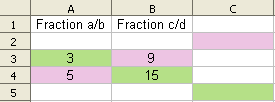
\includegraphics[width=.5\linewidth]{actiTableur}
\end{center}

\item Programme en \texttt{C2} le produit de \texttt{A4} par \texttt{B3} et en \texttt{C5} le produit de \texttt{A3} par \texttt{B4}.
\item Teste dans le tableur les trois fractions trouvées à la question 1. Que remarques-tu dans les cellules \texttt{C2} et \texttt{C5} ?
\item En te servant du tableur, trouve parmi les nombres en écriture fractionnaire suivants ceux qui sont égaux à $\dfrac{3}{5}$ : $\dfrac{301}{501}$ ; $\dfrac{192}{320}$ ; $\dfrac{8,1}{13,5}$ ; $\dfrac{2500}{4000}$.
\item Un nombre en écriture fractionnaire égal à $\dfrac{3}{5}$ s'écrit sous la forme $\dfrac{3\,k}{5\,k}$ où $k$ est un nombre non nul. Démontre que leurs produits en croix sont égaux.
\item On veut déterminer la fraction de dénominateur 120 égale à la fraction $\dfrac{3}{5}$. Remplis les cellules du tableur que l'on connaît et programme en \texttt{B3} le nombre cherché.
\item De la même façon, trouve les nombres manquants : $\dfrac{3}{5}=\dfrac{...}{75}$ ; $\dfrac{3}{5}=\dfrac{...}{125}$ ; $\dfrac{3}{5}=\dfrac{...}{0,25}$.
\end{enumerate}
\end{activite}


%%%%%%%%%%%%%%%%%%%%%%%%%%%%%%%%%%%%%%%%%%%%%%%


\begin{activite}[Inverses]
\begin{enumerate}
\item Quelle est la longueur du côté d'un carré d'aire 1 unité d'aire (U.A.) ?
\item On considère plusieurs rectangles qui ont tous la même aire de 1 U.A.. Recopie puis complète le tableau suivant par les nombres qui conviennent :
 
\renewcommand*\tabularxcolumn[1]{>{\centering\arraybackslash}m{#1}}
\renewcommand{\arraystretch}{1.6}
\begin{CLtableau}{\linewidth}{7}{c}
\hline
& Rectangle 1 & Rectangle 2 & Rectangle 3 & Rectangle 4 & Rectangle 5 & Rectangle 6 \\ \hline
Longueur & 2 & & & 3 & & $\dfrac{4}{3}$ \\ \hline
Largeur & & $0,1$ & $0,25$ & & $\dfrac{1}{7}$ & \\ \hline
\end{CLtableau}

    \begin{enumerate}
        \item Que dire de la longueur de ces rectangles ? Et de la largeur ?
        \item Quel lien y a-t-il entre la longueur et la largeur de ces rectangles ?
        
        \textbf{On dit que deux nombres sont inverses l'un de l'autre quand leur produit est égal à 1.}
        
        \item Recopie et complète : les nombres 2 et ... sont inverses l'un de l'autre, ainsi que $0,1$ et ... ; $0,25$ et ... ; 3 et ... ; $\dfrac{1}{7}$ et ... ; $\dfrac{4}{3}$ et ... .
        
        Que peux-tu dire pour le nombre 1 ?
        
        \item Soit $x$ un nombre non nul, quel est l'inverse de $x$ ? Justifie.
        \item Soient $a$ et $b$ deux nombres non nuls, quel est l'inverse de $\dfrac{a}{b}$ ? Justifie.
    \end{enumerate}
 
\end{enumerate}
\end{activite}



%%%%%%%%%%%%%%%%%%%%%%%%%%%%%%%%%%%%%%%%%%%%%%%



\begin{activite}[Comparaison dans tous les cas]

\begin{partie}[Dénominateurs n'ayant pas de diviseur commun autre que 1]
Corentin le lapin et Luce la puce décident de faire une course. Corentin fait des bonds de $\dfrac{1}{3}$ de mètre tandis que Luce fait des bonds de $\dfrac{1}{5}$ de mètre. 

\begin{center}
    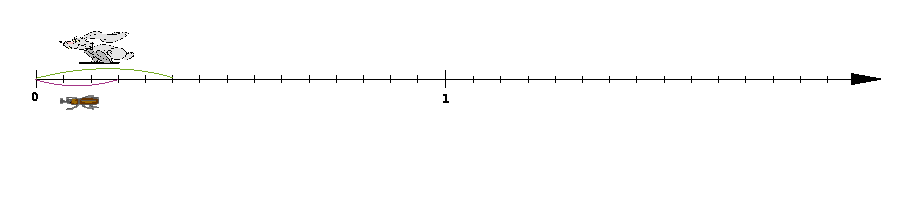
\includegraphics[width=\linewidth]{actiLapinScara}
\end{center}

    \begin{enumerate}
        \item Quand Corentin fait deux bonds, Luce en fait trois. Reproduis la demi-droite graduée ci-dessus représentant la course, puis place les points $C$ et $L$ pour indiquer les positions de Corentin et de Luce.
        \item Complète les phrases suivantes :
        
« Corentin a parcouru $\dfrac{...}{...}$ de mètre, ce qui équivaut à $\dfrac{...}{15}$ de mètre. »

« Luce a parcouru $\dfrac{...}{...}$ de mètre, ce qui équivaut à $\dfrac{...}{15}$ de mètre. »

        \item En t'aidant de la question 2, indique lequel des deux a parcouru la plus grande distance. Parmi les fractions $\dfrac{2}{3}$ et $\dfrac{3}{5}$, laquelle est la plus grande ?
    \end{enumerate}
\end{partie}

\begin{partie}[Dénominateurs ayant plusieurs diviseurs communs]
Lola la tortue et Jeannot le lièvre décident de faire une course sur une demi-droite graduée. Le point de départ est l'origine de la demi-droite. Lola parcourt $\dfrac{5}{4}$ d'unité et Jeannot parcourt $\dfrac{7}{6}$ d'unité.
    \begin{enumerate}
        \item Trace une demi-droite et gradue-la pour y placer les points $L$ et $J$ indiquant les positions de Lola et Jeannot.
        \item Lequel des deux a parcouru le plus grand trajet ? Parmi les fractions $\dfrac{5}{4}$ et $\dfrac{7}{6}$, laquelle est la plus grande ?
    \end{enumerate}
\end{partie}


\begin{partie}[Bilan]
\begin{enumerate}
    \item Énonce une règle qui permet de comparer des fractions de dénominateurs différents.
    \item Applique la règle que tu as trouvée pour comparer : $\dfrac{7}{5}$ et $\dfrac{13}{11}$ puis $\dfrac{3}{25}$ et $\dfrac{1}{10}$.
\end{enumerate}
\end{partie}

\end{activite}

%%%%%%%%%%%%%%%%%%%%%%%%%%%%%%%%%%%%%%%%%%%%%%%


\begin{activite}[Divisions]
\begin{enumerate}
\item Sachant que pour tous nombres $a$ et $b$ non nuls : $\dfrac{a}{b}=a \times \dfrac{1}{b}$, décompose de la même façon le quotient $\dfrac{\dfrac{3}{2}}{\dfrac{5}{3}}$.
\item Que peux-tu dire du nombre $\dfrac{1}{\dfrac{5}{3}}$ ? Déduis-en une fraction égale à ce nombre.
\item Transforme alors le quotient $\dfrac{\dfrac{3}{2}}{\dfrac{5}{3}}$ en produit et complète la phrase suivante : \emph{« Diviser par une fraction, c'est ... .».}
\item Termine alors le calcul du quotient de $\dfrac{3}{2}$ par $\dfrac{5}{3}$.
\item Applique cette règle pour effectuer les calculs suivants : $\dfrac{\dfrac{10}{11}}{\dfrac{7}{8}}$ ; $\dfrac{\dfrac{4}{7}}{\dfrac{5}{9}}$ ; $\dfrac{\dfrac{2}{5}}{\dfrac{14}{3}}$.
\end{enumerate}
\end{activite}


\cours
\section{Amplifier ou réduire un quotient}

\begin{aconnaitre}
\textbf{Si on multiplie ou si on divise} le numérateur et le dénominateur d'un quotient par \textbf{un même nombre non nul} alors on obtient \textbf{quotient égal}.

Pour tous nombres $a$, $b$ et $k$ où $b$ et $k$ sont non nuls :
\[ \frac{a \times k}{b \times k} = \frac{a}{b} \text{ et } \frac{a \div k}{b \div k} = \frac{a}{b}\]
\end{aconnaitre}

\begin{exemple*1}
Simplifie le quotient $\dfrac{42}{-140}$.
\correction

\begin{tabular}{lll}
$\dfrac{42}{-140}=-\dfrac{42}{140}$ & $\longrightarrow$ & On détermine le signe du quotient. \\
$\dfrac{42}{-140}=-\dfrac{3 \times 2 \times 7}{10 \times 7 \times 2}$  & $\longrightarrow$ & On cherche les facteurs communs à 2 et 140. \\
$\dfrac{42}{-140}=-\dfrac{3}{10}$ & $\longrightarrow$ & On simplifie le quotient. \\
\end{tabular}
\end{exemple*1}

\begin{exemple*1}
Détermine le nombre manquant dans l'égalité $\dfrac{-1,2}{6}=\dfrac{...}{18}$.
\correction

\vspace{.5em}
\begin{tabular}{lll}
\hspace{1.5em}
\includegraphics[width=.8cm]{figX3} & & \\
$\dfrac{-1,2}{6}=\dfrac{...}{18}$ & $\longrightarrow$ & Pour passer de 6 à 18 \textbf{on multiplie par 3}. \\
\hspace{1.5em}
\includegraphics[width=.8cm]{figX3b} & & \\
donc $\dfrac{-1,2}{6}=\dfrac{-3,6}{18}$  & $\longrightarrow$ & Ainsi, pour trouver le nombre manquant, \textbf{on multiplie} \\
& & \textbf{$\mathbf{-1,2}$ par 3}, ce qui donne $-3,6$. \\
\end{tabular}
\end{exemple*1}


\section{Comparer deux fractions}

\begin{aconnaitre}[Fractions dont le numérateur et le dénominateur sont positifs]
\begin{itemize}
\item Si les deux fractions ont le même dénominateur, la plus grande est celle qui a le plus grand numérateur.

Par exemple $\dfrac{5}{7}>\dfrac{2}{7}$ car $5 > 2$.

\item Si les deux fractions ont le même numérateur, la plus grande est celle qui a le plus petit dénominateur.

Par exemple $\dfrac{4}{9}<\dfrac{4}{5}$ car $9 > 5$.

\item Si une fraction est plus grande que 1 (son numérateur est plus grand que son dénominateur), alors elle est plus grande qu'une fraction qui est plus petite que 1 (dont le numérateur est plus petit que le dénominateur).

Par exemple $\dfrac{9}{5}>\dfrac{6}{7}$ car $\dfrac{9}{5}>1$ et $\dfrac{6}{7}<1$. 
\end{itemize}
\end{aconnaitre}



\begin{remarque}
Attention, les règles données ci-dessus ne sont pas vraies si le numérateur ou le dénominateur d'une des fractions est négatif.
\end{remarque}

\section{Multiplication}

\begin{aconnaitre}
Pour \textbf{multiplier des nombres en écriture fractionnaire}, on multiplie les numérateurs entre eux et les dénominateurs entre eux.

Pour tous nombres $a$, $b$, $c$ et $d$ où $b$ et $d$ sont non nuls :
\[ \dfrac{a}{b} \times \dfrac{c}{d} = \dfrac{a\times c}{b \times d} \]
\end{aconnaitre}

\begin{remarque}
Si $b=1$, la formule devient $a \times \dfrac{c}{d} = \dfrac{a\times c}{d}$
\end{remarque}

\begin{exemple*1}
Calcule l'expression $B=-\dfrac{35}{33} \times \dfrac{-39}{-80}$. Donne le résultat sous forme simplifiée.
\correction
\vspace{.5em}
 
\begin{tabular}{lll}
$B = -\dfrac{35 \times 39}{33 \times 80}$ & $\longrightarrow$ & On détermine le signe du résultat. \\
$B = -\dfrac{7 \times \mathbf{5} \times 13 \times \mathbf{3}}{11 \times \mathbf{3} \times 2 \times \mathbf{5} \times 8}$ & $\longrightarrow$ & On cherche des facteurs communs. \\
$B = -\dfrac{7 \times 13}{11 \times 2 \times 8}$ & $\longrightarrow$ & On simplifie. \\
$B = -\dfrac{91}{176}$ & $\longrightarrow$ & On calcule. \\
\end{tabular}
\end{exemple*1}

\section{Division de deux quotients}

\subsection{Inversion d'un nombre non nul}

\begin{definition}
\textbf{Deux nombres sont \MotDefinition{inverses}{}} l'un de l'autre si leur produit est égal à 1.
\end{definition}

\begin{propriete}
\begin{itemize}
    \item Tout nombre $x$ non nul admet un inverse qui est le nombre $\dfrac{1}{x}$.
    \item Tout nombre en écriture fractionnaire $\dfrac{a}{b}$ ($a\neq 0$ et $b \neq 0$) admet un inverse qui est le nombre $\dfrac{b}{a}$.
\end{itemize}
\end{propriete}

\begin{remarque}
\begin{itemize}
    \item Un nombre et son inverse ont toujours le même signe.
    
    En effet, leur produit 1 est positif et seul le produit de deux nombres de même signe est positif.
    \item Zéro est le seul nombre qui n'admet pas d'inverse.
    
    En effet, tout nombre multiplié par 0 donne 0 et ne donnera jamais 1.
\end{itemize}
\end{remarque}

\begin{exemple}
Calcule l'inverse de 3.
\correction
L'inverse de 3 est $\dfrac{1}{3}$.
\end{exemple}

\begin{exemple}
Calcule l'inverse de $\dfrac{-7}{3}$.
\correction
L'inverse de $\dfrac{-7}{3}$ est $\dfrac{1}{\dfrac{-7}{3}}=\dfrac{3}{-7}=\dfrac{-3}{7}$.
\end{exemple}

\subsection{Diviser des quotients}

\begin{aconnaitre}
\textbf{Diviser par un nombre non nul} revient à multiplier par l'inverse de ce nombre.

Pour tous nombres $a$, $b$, $c$ et $d$ où $b$, $c$ et $d$ sont non nuls :
\[ \dfrac{a}{b} \div \dfrac{c}{d} = \dfrac{a}{b} \times \dfrac{d}{c} \text{ ou } \dfrac{\phantom{i}\dfrac{a}{b}\phantom{i}}{\dfrac{c}{d}}=\dfrac{a}{b} \times \dfrac{d}{c} \]
\end{aconnaitre}

\begin{exemple*1}
Calcule $C=\dfrac{-8}{7} \div \dfrac{5}{-3}$.
\correction
\vspace{.5em}
 
\begin{tabular}{lll}
$C=+\left(\dfrac{8}{7} \div \dfrac{5}{3}\right)$ & $\longrightarrow$ & On détermine le signe du résultat. \\
$C=\dfrac{8}{7} \times \dfrac{3}{5}$ & $\longrightarrow$ & On multiplie par l'inverse du deuxième quotient. \\
$C=\dfrac{8\times 3}{7\times 5}$ & $\longrightarrow$ & On multiplie les fractions. \\
$C=\dfrac{24}{35}$ & $\longrightarrow$ & On calcule. \\
\end{tabular}
\end{exemple*1}


\begin{exemple*1}
Calcule $D=\dfrac{-\dfrac{32}{21}}{\dfrac{-48}{-35}}$ et donne le résultat en le simplifiant le plus possible.
\correction
\vspace{.5em}
 
\begin{tabular}{lll}
$D=-\dfrac{\dfrac{32}{21}}{\dfrac{48}{35}}$ & $\longrightarrow$ & On détermine le signe du résultat. \\
$D=-\dfrac{32}{21}\times \dfrac{35}{48}$ & $\longrightarrow$ & On multiplie par l'inverse du deuxième quotient. \\
$D=-\dfrac{\mathbf{8}\times \mathbf{2}\times 2 \times \mathbf{7} \times 5}{\mathbf{7 \times 3 \times 3 \times \mathbf{2} \times \mathbf{8}}}$ & $\longrightarrow$ & On cherche des facteurs communs. \\
$D=-\dfrac{10}{9}$ & $\longrightarrow$ & On calcule sans oublier de simplifier avant ! \\
\end{tabular}
\end{exemple*1}


\begin{exemple*1}
Quelle est la nature du nombre $E$ défini par $E=\dfrac{1+\dfrac{2}{3}}{1-\dfrac{2}{3}}$ ?
\correction
\vspace{.5em}
 
\begin{tabular}{lll}
$E=\dfrac{\dfrac{3}{3}+\dfrac{2}{3}}{\dfrac{3}{3}-\dfrac{2}{3}}=\dfrac{\dfrac{5}{3}}{\dfrac{1}{3}}$ & $\longrightarrow$ & $E$ peut s'écrire aussi $E=\left(1+\dfrac{2}{3}\right) \div \left(1-\dfrac{2}{3}\right)$. \\
 & & On commence donc par calculer les parenthèses.\\
$E=\dfrac{5}{3} \times \dfrac{3}{1}$ & $\longrightarrow$ & On multiplie par l'inverse du deuxième quotient. \\
$E=\dfrac{5\times \mathbf{3}}{\mathbf{3}\times 1}$ & $\longrightarrow$ & On cherche des facteurs communs. \\
$E=5$ donc $E$ est un nombre entier. & &  \\
\end{tabular}
\end{exemple*1}


\section{Signe d'une fraction}

\begin{propriete}
Pour déterminer le signe d'une fraction, on utilise la règle du produit des signes.
\end{propriete}

\begin{aconnaitre}
Si une fraction est négative, on peut l'écrire de trois manières différentes en mettant le signe moins au numérateur, au dénominateur (peu utilisé) ou devant la fraction.
On écrira donc indifféremment  $\dfrac{-2}{3}$ ou $-\dfrac{2}{3}$ et rarement $\dfrac{2}{-3}$.
\end{aconnaitre}



\exercicesbase
\begin{colonne*exercice}
\serie{Comparaison}


\begin{exercice}[Signes]
Donne le signe des nombres suivants :

$\dfrac{-5,2}{4,23}$ ; $\dfrac{5}{-2,1}$ ; $\dfrac{472}{23}$ ; $\dfrac{-8,9}{-45}$ ; $-\dfrac{12}{13}$ ; $-\dfrac{11}{-5,2}$.
\end{exercice}





\begin{exercice}
Indique les nombres égaux parmi ceux de la liste ci-dessous :

$\dfrac{-8}{9}$ ; $-\dfrac{8}{9}$ ; $\dfrac{-8}{-9}$ ; $-\dfrac{8}{-9}$ ; $\dfrac{8}{-9}$ ; $-\dfrac{-8}{9}$ ; $\dfrac{8}{9}$.
\end{exercice}




\begin{exercice}[Encadrement]

\begin{enumerate}
\item On considère la fraction $\dfrac{56}{21}$.

Effectue la division euclidienne de 56 par 21 et déduis-en un encadrement de la fraction par deux nombres entiers consécutifs.
\item Encadre $\dfrac{-89}{15}$ puis $\dfrac{47}{59}$ par deux nombres entiers consécutifs.
\item Encadre respectivement $\dfrac{-47}{25}$ et $\dfrac{13}{-4}$ par deux nombres entiers consécutifs et déduis-en la comparaison de ces deux fractions.
\item Peux-tu appliquer la même méthode pour comparer $\dfrac{25}{3}$ et $\dfrac{90}{11}$ ?
\end{enumerate}
\end{exercice}




\begin{exercice}[Avec des valeurs approchées]
Soient deux nombres : $a =\dfrac{816}{577}$  et $b =\dfrac{577}{408}$.
\begin{enumerate}
\item Donne la valeur arrondie de $a$ et celle de $b$ au millième. Peux-tu en déduire la comparaison de $a$ et de $b$ ?
\item Donne des valeurs approchées de $a$ et $b$ qui permettent de les comparer. Compare $a$ et $b$.
\end{enumerate}
\end{exercice}





\begin{exercice}[Égalités]
Recopie et complète chacune des égalités suivantes :
\begin{enumerate}
\item $\dfrac{...}{-5}=\dfrac{10}{20}$
\item $\dfrac{2}{3}=\dfrac{...}{27}$
\item $\dfrac{-15}{45}=\dfrac{-5}{...}$
\item $\dfrac{...}{-18}=\dfrac{7}{6}$
\item $3=\dfrac{...}{4}$
\item $-2,1=-\dfrac{21}{...}$
\end{enumerate}
\end{exercice}




\begin{exercice}
Dans chaque cas, à partir des égalités données et en utilisant seulement les quatre nombres qui apparaissent, écris toutes les égalités d'écritures fractionnaires possibles :
\begin{enumerate}
\item $7 \times (-8) = -4 \times 14$
\item $-3 \times (-1) = 2 \times 1,5$
\item $2,1 \times 12 = 9 \times 2,8$
\item $-4 \times 9 = 12 \times (-3)$
\end{enumerate}
\end{exercice}




\begin{exercice}[Égalité ?]
Recopie et complète en utilisant $=$ ou $\neq$, en justifiant dans chaque cas :
\begin{enumerate}
\item $\dfrac{9}{5} ... \dfrac{26}{15}$ 
\item $\dfrac{-7}{-3} ... \dfrac{-14}{6}$
\item $\dfrac{-12,7}{-5} ... \dfrac{25,4}{10}$
\item $\dfrac{-27,35}{27,35} ... \dfrac{15,72}{-15,72}$
\end{enumerate}
\end{exercice}





\begin{exercice}[Avec un dénominateur entier positif]
Réécris chacune des écritures fractionnaires suivantes avec un dénominateur entier positif :
$\dfrac{4}{-5}$ ; $\dfrac{-8}{-7}$ ; $-\dfrac{5,2}{-7}$ ; $\dfrac{7}{-2,1}$ ; $\dfrac{8,2}{0,12}$ ; $-\dfrac{-1}{-3,54}$.
\end{exercice}





\begin{exercice}[Même dénominateur positif]
\begin{enumerate}
\item Recopie et complète la phrase suivante :

« Deux nombres en écriture fractionnaire de même dénominateur positif sont rangés... ».
\item Compare les nombres suivants :

$\dfrac{-7,5}{3}$ et $\dfrac{-7,49}{3}$ ;

$\dfrac{4,05}{2,1}$ et $\dfrac{4,2}{2,1}$ ;

$-\dfrac{0,74}{5}$ et $\dfrac{-0,7309}{5}$ ; 

$\dfrac{8}{-5,23}$ et $\dfrac{-7,9}{5,23}$. 
\end{enumerate}
\end{exercice}





\begin{exercice}[Avec le même numérateur]
\begin{enumerate}
\item Recopie et complète la phrase suivante :

« Deux nombres positifs en écriture fractionnaire de même numérateur sont rangés… »
\item Compare les nombres suivants :

$\dfrac{3,5}{8,2}$ et $\dfrac{3,5}{8,15}$ ;

$-\dfrac{-1}{6}$ et $\dfrac{1}{5,7}$.
\end{enumerate}
\end{exercice}




\begin{exercice}[Avec le même numérateur (bis)]
Compare les nombres suivants en commençant par comparer leurs opposés :
\begin{enumerate}
\item $\dfrac{1}{-5}$ et $\dfrac{1}{-7}$ ;
\item $\dfrac{-3}{8}$ et $\dfrac{-3}{8,2}$ ;
\item $-\dfrac{5,23}{14,5}$ et $\dfrac{-5,23}{14,6}$ ;
\item $\dfrac{-7,5}{0,23}$ et $\dfrac{75}{-2,4}$. 
\end{enumerate}
\end{exercice}





\begin{exercice}
Dans chaque cas, réécris les nombres avec le même dénominateur positif puis compare-les :
\begin{enumerate} 
\item $\dfrac{-5}{4}$ et $\dfrac{-9}{8}$ ;
\item $\dfrac{2,7}{-9}$ et $\dfrac{-1}{3}$ ;
\item -3 et $-\dfrac{20,9}{-7}$ ;
\item $-\dfrac{2}{11}$ et $\dfrac{-5}{33}$ ; 
\item $\dfrac{7}{2,5}$ et $\dfrac{-20,5}{7,5}$ ; 
\item $\dfrac{13}{-27}$ et $\dfrac{-79}{162}$.
\end{enumerate}
\end{exercice}




\begin{exercice}[Multiple commun]
\begin{enumerate}
\item Quels sont les dix premiers multiples de 12 ? Ceux de 18 ? Déduis-en le plus petit multiple non nul commun à 12 et 18, puis un dénominateur commun positif des fractions : $\dfrac{-7}{12}$ et $\dfrac{-11}{18}$.

Compare alors ces deux nombres.
\item La méthode précédente permet-elle de trouver rapidement un dénominateur commun aux nombres : $\dfrac{8}{11}$ et $\dfrac{10}{13}$ ?

Comment en trouver un alors rapidement ? Compare ces deux nombres.
\end{enumerate}
\end{exercice}





\begin{exercice}Dans chaque cas, réécris les nombres avec le même dénominateur positif, puis compare-les :
\begin{enumerate}
\item $\dfrac{-5}{8}$ et $\dfrac{-3,8}{6}$ ;
\item $\dfrac{14}{5}$ et $\dfrac{20}{7}$ ;
\item $\dfrac{3}{-50}$ et $-\dfrac{4}{75}$ ;
\item $\dfrac{54,5}{0,27}$ et $\dfrac{-2,62}{0,13}$.
\end{enumerate}
\end{exercice}






\begin{exercice}
Compare en justifiant :
\begin{enumerate}
\item $-\dfrac{12}{18}$ et $\dfrac{399}{-300}$ ; 
\item $\dfrac{2}{57}$ et $\dfrac{1}{28,4}$ ;
\item $\dfrac{-75}{47}$ et $\dfrac{25}{-15}$ ;
\item $\dfrac{-5}{6}$ et $-\dfrac{15}{14}$ ;
\item $\dfrac{6}{13}$ et $\dfrac{29}{65}$ ;
\item $\dfrac{3}{-22}$ et $\dfrac{4,5}{33}$.
\end{enumerate}
\end{exercice}




\begin{exercice}[Dans l'ordre]
\begin{enumerate}
\item Range les nombres suivants dans l'ordre croissant sans utiliser de valeurs approchées :

$\dfrac{7}{-15}$ ; $\dfrac{7}{3}$ ; $\dfrac{490}{420}$ ; $\dfrac{-5}{12}$ ; $\dfrac{-24}{-18}$ ; 2,5.
\item Range les nombres suivants dans l'ordre décroissant :

$\dfrac{-29}{100}$ ; $\dfrac{7}{-25}$ ; $-0,285$ ; $-\dfrac{1}{5}$ ; $\dfrac{13}{-50}$ ; 0 ; $\dfrac{-1}{2,5}$.
\end{enumerate}
\end{exercice}





\begin{exercice}[Trajet]
Quatre amis font un voyage en trois jours. Le premier jour, ils parcourent 40\,\%\ du trajet total ; le deuxième jour, un quart et le dernier jour, $\dfrac{7}{20}$ du trajet total.

Quel jour ont-ils parcouru la plus grande distance ?

Peux-tu calculer la distance parcourue chaque jour ?
\end{exercice}







\serie{Multiplications}





\begin{exercice}[La règle et les signes]
Effectue les produits suivants :
\begin{enumerate}
\item $\dfrac{3}{2} \times \dfrac{5}{7}$ ;
\item $\dfrac{-4}{11} \times \dfrac{1}{-3}$ ;
\item $3 \times \dfrac{-7}{5}$ ;
\item $\dfrac{5}{-4} \times \dfrac{5}{-2}$ ;
\item $\dfrac{8}{17} \times \dfrac{5}{-3}$ ;
\item $-\dfrac{13}{5} \times \left(-\dfrac{2}{11}\right)$ ;
\item $\left(-\dfrac{7}{15}\right) \times (-8) \times \dfrac{2}{3}$ ;
\item $\dfrac{-1}{2} \times \dfrac{5}{-4} \times \dfrac{-3}{2}$.
\end{enumerate}
\end{exercice}





\begin{exercice}[Toujours plus simple]
Simplifie, si possible, les écritures fractionnaires suivantes :
\begin{enumerate}
\item $\dfrac{-5 \times 2}{2 \times 7}$ ;  
\item $\dfrac{-5 + 2}{7 + 2}$ ;
\item $\dfrac{4 \times (-11)}{4 \times (-11) \times 3}$ ;
\item $\dfrac{8 \times (-3) \times 7 \times 5}{3 \times 5 \times 8 \times 7}$ ;
\item $\dfrac{-5 \times 8}{2 \times (-7)}$ ;
\item $\dfrac{5 \times (-9) \times 2}{(-7) \times 10 \times (-1)}$ ;
\end{enumerate}
\end{exercice}





\begin{exercice}[Calculer en simplifiant]
Pour chacun des produits suivants, applique la règle de multiplication sans effectuer les calculs, simplifie lorsque cela est possible et donne alors le résultat sous la forme d'une fraction irréductible :
\begin{enumerate}
\item $\dfrac{8}{5} \times \dfrac{5}{7}$ ;
\item $\dfrac{-3}{10} \times \dfrac{-11}{3}$ ;
\item $\dfrac{-2}{3} \times \dfrac{-5}{2} \times \dfrac{3}{-7}$ ;
\item $\dfrac{5}{-7} \times \left(-\dfrac{7}{5}\right)$ ;
\item $-15 \times \dfrac{2}{15}$ ;
\item $\left(-\dfrac{8}{3}\right) \times \left(-\dfrac{1}{5}\right) \times 3$.
\end{enumerate}
\end{exercice}




\begin{exercice}Complète les égalités  suivantes :
\begin{enumerate}
\item $\dfrac{8}{...} \times \dfrac{7}{3} = -\dfrac{8}{3}$ ; 
\item $\dfrac{-5}{3} \times \dfrac{7}{...} = \dfrac{7}{6}$ ;
\item $\dfrac{6}{5} \times ... = -6$ ;
\item $\left(-\dfrac{8}{21}\right) \times \dfrac{...}{...} = 1$ ;
\item $\dfrac{...}{10} \times \dfrac{7}{...} = -5$ ;
\item $\dfrac{...}{-9} \times \dfrac{2}{...} = \dfrac{4}{15}$ ;
\item $\dfrac{-5}{...} \times \dfrac{3}{-14} \times \dfrac{...}{25} = \dfrac{-2}{7}$.
\end{enumerate}
\end{exercice}




\begin{exercice}[Simplifier avant de calculer]
\begin{enumerate}
\item Écris 15 sous la forme d'un produit de deux nombres entiers. Décompose de même 20 en produit de nombres entiers positifs les plus petits possibles.
\item Recopie et complète les égalités suivantes :
$\dfrac{15}{7} \times \dfrac{11}{20} = \dfrac{... \times ...}{... \times ...} = \dfrac{(... \times ...) \times ...}{... \times (... \times ... \times ...)}$.
\item Simplifie l'expression obtenue et donne le résultat sous forme d'une fraction irréductible.
\end{enumerate}
\end{exercice}





\begin{exercice}
Calcule les produits suivants en simplifiant, puis donne les résultats sous la forme d'une fraction irréductible :
\begin{enumerate}
\item $\dfrac{-7}{25} \times \dfrac{-5}{8}$ ;
\item $\dfrac{18}{-49} \times \dfrac{14}{27}$ ;
\item $\dfrac{45}{28} \times \dfrac{7}{-15}$ ;
\item $\dfrac{-2}{6} \times \left(-\dfrac{21}{11}\right)$ ;
\item $\dfrac{21}{32} \times \dfrac{108}{49}$ ;
\item $-26 \times \dfrac{-5}{39}$ ;
\item $\dfrac{8}{5} \times \dfrac{-5}{21} \times \left(-\dfrac{9}{16}\right)$ ;
\item $\dfrac{56}{-5} \times \dfrac{30}{21} \dfrac{7}{10}$.
\end{enumerate}
\end{exercice} 




\begin{exercice}[Avec la calculatrice]
Utilise ta calculatrice pour effectuer les produits suivants et donne les résultats sous la forme d'une fraction irréductible :
\begin{enumerate}
\item $\dfrac{686}{-153} \times \dfrac{-99}{-196}$ ; 
\item $\dfrac{2,1}{12,5} \times \left(-\dfrac{6,25}{0,49}\right)$.
\end{enumerate}
\end{exercice}



\begin{exercice}
Calcule mentalement :
\begin{enumerate}
\item les trois quarts de 400 ;
\item le double de $\dfrac{-7}{15}$ ;
\item les cinq septièmes des six cinquièmes de l'unité ;
\item les $\dfrac{7}{10}$ de $\dfrac{9}{10}$.
\end{enumerate}
\end{exercice}




\begin{exercice}[Dépense]
Abdel dépense les $\dfrac{5}{12}$ de son argent de poche, puis les trois quarts de ce qu'il lui reste alors.
\begin{enumerate}
\item Quelle fraction de son argent de poche a-t-il dépensée la deuxième fois ?
\item Le montant de son argent de poche étant de 72\,€, combien a-t-il dépensé au total ?
\end{enumerate}
\end{exercice}



\begin{exercice}
Recopie et complète en utilisant $=$ ou $\neq$, en justifiant dans chaque cas :
\begin{enumerate}
\item $\dfrac{-9,1}{5,2} ... \dfrac{79,8}{-45,6}$ ;
\item $\dfrac{-5}{-3} ... \dfrac{-3,5}{2,1}$ ;
\item $\dfrac{17,36}{-22,32} ... -\dfrac{28,7}{36,9}$ ;
\item $\dfrac{-56}{-57} ... \dfrac{57}{58}$ ;
\end{enumerate}
\end{exercice}





\serie{Divisions}


\begin{exercice}Inverses
Recopie et complète les égalités suivantes et écris, dans chaque cas, trois phrases utilisant le mot « inverse(s) » :
\begin{enumerate}
\item $4 \times \dfrac{1}{...} = 1$ ;
\item $... \times 0,25 = 1$ ;
\item $\dfrac{1}{...} \times (-3) = 1$ ;
\item $... \times \left(-\dfrac{1}{15}\right) = 1$ ;
\item $\dfrac{3}{4} \times \dfrac{...}{...} = 1$ ;
\item $\dfrac{...}{-25} \times \dfrac{...}{7} = 1$ ;
\item $... \times \left(-\dfrac{8}{5}\right) = 1$ ;
\item $-0,01 \times ... = 1$
\end{enumerate}
\end{exercice}



\begin{exercice}[Ne pas confondre !]
\begin{enumerate}
\item Recopie et complète les égalités suivantes :
\[ \left(\dfrac{9}{-14}\right) \times ... = 1 et \left(\dfrac{9}{-14}\right) + ... = 0\].
Écris deux phrases, l'une utilisant le mot « opposé(s) » et l'autre, le mot « inverse(s) ».
\item Trouve deux nombres qui sont leur propre inverse. Trouve un nombre qui est son propre opposé.
\item Tous les nombres ont-ils un inverse ? Un opposé ?
\item Quel est l'opposé de l'inverse de 4 ? Quel est l'inverse de l'opposé de 4 ?
\end{enumerate}
\end{exercice}



\begin{exercice}[Inverse]
\begin{enumerate}
\item Recopie et complète le tableau ci-dessous avec des écritures fractionnaires.

\renewcommand*\tabularxcolumn[1]{>{\centering\arraybackslash}m{#1}}
\renewcommand{\arraystretch}{1.6}
\begin{Ctableau}{\linewidth}{7}{c}
\hline
$x$ & 7 & $\dfrac{-3}{5}$ & $-\dfrac{8}{9}$ & $-0,6$ & $1,25$ \\ \hline
$\dfrac{1}{x}$ & & & & & \\ \hline
\end{Ctableau}
\item Détermine l'inverse de l'inverse de chaque nombre. Que remarques-tu ?
\end{enumerate}
\end{exercice}


\begin{exercice}[Mentalement]
\begin{enumerate}
\item Effectue mentalement les calculs suivants : $16 \div 2$ ; $100 \times 0,25$ ; $16 \times 0,5$ ; $100 \div 4$.
\item Justifie les résultats égaux avec la règle de division.
\end{enumerate}
\end{exercice}


\begin{exercice}La règle
Applique dans chaque cas la règle de division puis effectue les calculs :
\begin{enumerate}
\item $\dfrac{2}{3} \div 5$ ; 
\item $\dfrac{-5}{7} \div (-4)$ ;
\item $\dfrac{5}{6} \div \dfrac{7}{-11}$ ;
\item $8 \div \dfrac{1}{8}$ ;
\item $\dfrac{-3}{2} \div \dfrac{-5}{7}$ ;
\item $\dfrac{1}{10} \div \left(-\dfrac{7}{9}\right)$.
\end{enumerate}
\end{exercice}

\begin{exercice}Trait de fraction
Écris les quotients suivants en utilisant le symbole $\div$ puis effectue le calcul :
\[ A = \dfrac{2}{\dfrac{3}{5}}  ; B = \dfrac{\dfrac{2}{3}}{5} ; C = \dfrac{\dfrac{2}{3}}{\dfrac{7}{11}}.\]
\end{exercice}


\begin{exercice}[Division et simplification]
Applique la règle de division, simplifie puis effectue les calculs et donne les résultats sous la forme d'une fraction irréductible :
\begin{enumerate}
\item $\dfrac{8}{-15} \div \dfrac{-4}{5}$ ;
\item $\dfrac{9}{10} \div (-3)$ ;
\item $\dfrac{-4}{45} \div \dfrac{16}{15}$ ;
\item $\dfrac{-5}{6} \div \left(-\dfrac{15}{18}\right)$ ;
\item $12 \div \dfrac{3}{-4}$ ;
\item $1 \div \left(\dfrac{-7}{4}\right)$.
\end{enumerate}
\end{exercice}

\end{colonne*exercice}


\exercicesappr
\begin{colonne*exercice}
%\begin{exercice}[Partage]
\begin{enumerate}
\item Calcule la moitié de $\dfrac{-5}{12}$.
\item Il reste les $\dfrac{7}{8}$ d'un gâteau.

Trois amis décident de se partager équitablement ce reste : quelle fraction du gâteau aura chacun d'entre eux ?
\end{enumerate}
\end{exercice}


\begin{exercice}[Avec des lettres]
\begin{enumerate}
\item Sachant que $a = \dfrac{-2}{21}$  et $b =\dfrac{5}{-7}$, calcule :
\[	\dfrac{a}{b} ; \dfrac{b}{a} ; a \times b ; a + b \text{ et } a - b\]
Tu donneras les résultats sous la forme d'une fraction irréductible.
\item Même consigne avec $a =\dfrac{5}{24}$  et $b =-\dfrac{35}{18}$.
\end{enumerate}
\end{exercice}


\begin{exercice}
Jenny avait 145 fr. Elle a dépensé les $\dfrac{2}{5}$ de ce qu'elle avait. Combien d’argent lui reste-t-il ?
\end{exercice}


\begin{exercice}
Un salarié gagne 3900 CHF par mois. Il dépense $\dfrac{3}{20}$ de cette somme pour son loyer, $\dfrac{1}{13}$ pour les impôts et 2000 CHF pour vivre. Combien économise-t-il chaque mois ?
\end{exercice}

\columnbreak
\begin{exercice}
J'ai dépensé les $\dfrac{4}{5}$ de mon argent pour acheter un livre qui coûtait 32 CHF. Quelle somme avais-je dans mon porte-monnaie?
\end{exercice}


\begin{exercice}
Olivier a les $\dfrac{7}{16}$ des $\dfrac{2}{3}$ de l'âge de sa mère qui a 48 ans. Quel est l’âge d’Olivier ?
\end{exercice}


\begin{exercice}
Pierre dit à sa sœur pour l'impressionner: « Ce livre a coûté très cher. Je l'ai payé $\dfrac{5}{12}$ des $\dfrac{6}{5}$ de 20 CHF. » Quel est le prix du livre ?
\end{exercice}


\begin{exercice}
Alicia et Alizée ont groupé leurs économies pour s’acheter un lecteur MP3 et des DVD. 

Elles ont dépensé les $\dfrac{6}{10}$ de leur pactole pour l'achat du lecteur MP3 et les $\dfrac{6}{9}$ de ce qu'il restait pour l’acquisition des DVD. Après ces achats, il ne leur reste plus que 28 €.
\begin{enumerate}
\item De quelle somme disposaient-elles avant de faire leurs achats ? 
\item Quel est le prix du lecteur MP3 et celui des DVD ?
\end{enumerate}
\end{exercice}


\begin{exercice}
Monsieur Reesh avait 500 000 CHF dans son coffre mais Arsène Lupin est passé par là et lui a dérobé $\dfrac{3}{4}$ des $\dfrac{5}{6}$ des $\dfrac{4}{5}$ de la somme. Combien lui reste-t-il dans son coffre ?
\end{exercice}


\begin{exercice}
Lors de ses dernières vacances, Alex a dépensé les $\dfrac{3}{4}$ des $\dfrac{5}{9}$ des $\dfrac{7}{10}$ de son argent de poche qui se montait à 3000 CHF. Quelle somme lui reste-t-il ?
\end{exercice}


\end{colonne*exercice}

\connaissances
%\QCMautoevaluation{Pour chaque question, plusieurs réponses sont proposées. Déterminer celles qui sont correctes.}

\begin{QCM}
\begin{GroupeQCM}

\begin{exercice}
La valeur arrondie au dixième de $\dfrac{2}{3}$ est...
\begin{ChoixQCM}{4}
\item $0$
\item $1$
\item $0,6$
\item $0,7$
\end{ChoixQCM}
\begin{corrige}
\reponseQCM{a}
\end{corrige}
\end{exercice}

\begin{exercice}
Une valeur approchée de $\dfrac{19}{13}$ au millième près est...
\begin{ChoixQCM}{4}
\item $1,46$
\item $1,461$
\item $1,462$
\item $1,4615$
\end{ChoixQCM}
\begin{corrige}
\reponseQCM{a}
\end{corrige}
\end{exercice}


\begin{exercice}
$\dfrac{-24}{-18}=...$
\begin{ChoixQCM}{4}
\item $\dfrac{20}{15}$
\item $-\dfrac{4}{3}$
\item $1,33$
\item $\dfrac{4}{3}$
\end{ChoixQCM}
\begin{corrige}
\reponseQCM{a}
\end{corrige}
\end{exercice}


\begin{exercice}
L'opposé de $\dfrac{4}{5}$ est...
\begin{ChoixQCM}{4}
\item $\dfrac{5}{4}$
\item $\dfrac{-4}{-5}$
\item $\dfrac{-4}{5}$
\item $-\dfrac{4}{5}$
\end{ChoixQCM}
\begin{corrige}
\reponseQCM{a}
\end{corrige}
\end{exercice}


\begin{exercice}
$\left(\dfrac{4}{5}\right)^{-1} = ...$
\begin{ChoixQCM}{4}
\item $\dfrac{3}{5}$
\item $\dfrac{-4}{-5}$
\item $\dfrac{5}{4}$
\item $-\dfrac{4}{5}$
\end{ChoixQCM}
\begin{corrige}
\reponseQCM{a}
\end{corrige}
\end{exercice}


\end{GroupeQCM}


\begin{GroupeQCM}

\begin{exercice}
$\dfrac{37}{15}$ est supérieur à...
\begin{ChoixQCM}{4}
\item $2$
\item $\dfrac{77}{30}$
\item $\dfrac{598}{599}$
\item $\dfrac{25}{10}$
\end{ChoixQCM}
\begin{corrige}
\reponseQCM{a}
\end{corrige}
\end{exercice}


\begin{exercice}
$\dfrac{-14}{5}$ est inférieur à...
\begin{ChoixQCM}{4}
\item $\dfrac{14}{-5}$
\item $-2$
\item $\dfrac{-14}{3}$
\item son inverse
\end{ChoixQCM}
\begin{corrige}
\reponseQCM{a}
\end{corrige}
\end{exercice}


\begin{exercice}
$\dfrac{-5}{6}$ est le résultat de...
\begin{ChoixQCM}{4}
\item $\dfrac{-1}{3} \times \dfrac{-5}{2}$
\item $\dfrac{-5}{11} \times \dfrac{11}{6}$
\item $\dfrac{-30}{36} \div 6$
\item $-5 \times \dfrac{1}{6}$
\end{ChoixQCM}
\begin{corrige}
\reponseQCM{a}
\end{corrige}
\end{exercice}


\begin{exercice}
$-\dfrac{7}{5} \div \dfrac{2}{-3}=...$
\begin{ChoixQCM}{4}
\item $2,1$
\item $\dfrac{10}{21}$
\item $\dfrac{3,5}{1,6}$
\item $-\dfrac{21}{10}$
\end{ChoixQCM}
\begin{corrige}
\reponseQCM{a}
\end{corrige}
\end{exercice}


\begin{exercice}
$\dfrac{\dfrac{2}{3}}{4}=...$
\begin{ChoixQCM}{4}
\item $2 \div 3 \div 4$
\item $\dfrac{8}{3}$
\item $\dfrac{2}{12}$
\item On ne peut pas calculer
\end{ChoixQCM}
\begin{corrige}
\reponseQCM{a}
\end{corrige}
\end{exercice}

\end{GroupeQCM}
\end{QCM}

\TravauxPratiques
%\begin{TP}[Dominos en fractions]


Vous allez créer un jeu de dominos utilisant des fractions.

\begin{enumerate}
    \item Répartissez-vous le travail pour compléter le tableau ci-dessous. La première ligne (cases A1 à F1) contient les résultats des calculs situés dans les lignes 2 à 7.

\vspace{1em}
\renewcommand*\tabularxcolumn[1]{>{\centering\arraybackslash}m{#1}}
\renewcommand{\arraystretch}{1.6}
\begin{cltableau}{\linewidth}{7}
\hline
 & A & B & C & D & E & F \\ \hline
1 & $\dfrac{5}{3}$ & $\dfrac{-3}{5}$ & $\dfrac{3}{5}$ & $\dfrac{-9}{4}$ & $\dfrac{2}{7}$ & $3$ \\ \hline
2 & $\dfrac{1}{3} + \dfrac{4}{3}$ & $\dfrac{-4}{5} +\dfrac{1}{5}$ & & & & \\ \hline
3 & $\dfrac{7}{3}-\dfrac{4}{6}$ & $\dfrac{2}{15}-\dfrac{1}{5}-\dfrac{8}{15}$ & & & & \\ \hline
4 & $\dfrac{2}{3}+1$ & $\dfrac{12}{5}-3$ & & & & \\ \hline
5 & & & & & & \\ \hline
6 & & & & & & \\ \hline
7 & & & & & & \\ \hline
\end{cltableau}

\vspace{1em}

Quelques exemples (cases A2, B2, A3, B3, A4, B4) ont été donnés à titre indicatif. Pour chaque colonne, il faut trouver :
\begin{itemize}
    \item ligne 2 : une somme algébrique de fractions de même dénominateur ;
    \item ligne 3 : une somme algébrique de fractions de dénominateurs différents ;
    \item ligne 4 : une somme algébrique d'un nombre entier et d'une fraction ;
    \item ligne 5 : un produit de deux fractions ;
    \item ligne 6 : un produit de trois fractions ;
    \item ligne 7 : un quotient de deux fractions.
\end{itemize}

    \item Créez le jeu de dominos en respectant le plan suivant (à chaque fois, il faut remplacer le nom de la case par son contenu).
    
    Taille d'un domino : 6\,cm sur 2\,cm.
    
    \vspace{1em}
    \begin{center}
        \renewcommand*\tabularxcolumn[1]{>{\centering\arraybackslash}m{#1}}
        \begin{tabularx}{.6\linewidth}{|X|X|X|X|X|X|X|X|}
        \cline{1-2} \cline{4-5} \cline{7-8}
            A1 & A2 & & A3 & B1 & & A4 & C2 \\ \cline{1-2} \cline{4-5} \cline{7-8}
        \end{tabularx}
        \vspace{.5em}
        
        \begin{tabularx}{.6\linewidth}{|X|X|X|X|X|X|X|X|}
        \cline{1-2} \cline{4-5} \cline{7-8}
            A5 & D3 & & A6 & E4 & & A7 & F5 \\ \cline{1-2} \cline{4-5} \cline{7-8}
        \end{tabularx}
        \vspace{.5em}
        
        \begin{tabularx}{.6\linewidth}{|X|X|X|X|X|X|X|X|}
        \cline{1-2} \cline{4-5} \cline{7-8}
            B2 & B3 & & B4 & C1 & & B5 & D2 \\ \cline{1-2} \cline{4-5} \cline{7-8}
        \end{tabularx}
        \vspace{.5em}
        
        \begin{tabularx}{.6\linewidth}{|X|X|X|X|X|X|X|X|}
        \cline{1-2} \cline{4-5} \cline{7-8}
            B6 & E3 & & B7 & F4 & & C3 & C4 \\ \cline{1-2} \cline{4-5} \cline{7-8}
        \end{tabularx}
        \vspace{.5em}
        
        \begin{tabularx}{.6\linewidth}{|X|X|X|X|X|X|X|X|}
        \cline{1-2} \cline{4-5} \cline{7-8}
            C5 & D1 & & C6 & E2 & & C7 & F3 \\ \cline{1-2} \cline{4-5} \cline{7-8}
        \end{tabularx}
        \vspace{.5em}
        
        \begin{tabularx}{.6\linewidth}{|X|X|X|X|X|X|X|X|}
        \cline{1-2} \cline{4-5} \cline{7-8}
            D4 & D5 & & D6 & E1 & & D7 & F2 \\ \cline{1-2} \cline{4-5} \cline{7-8}
        \end{tabularx}
        \vspace{.5em}
        
        \begin{tabularx}{.6\linewidth}{|X|X|X|X|X|X|X|X|}
        \cline{1-2} \cline{4-5} \cline{7-8}
            E5 & E6 & & E7 & F1 & & F6 & F7 \\ \cline{1-2} \cline{4-5} \cline{7-8}
        \end{tabularx}
    \end{center}
    
    \item Découpez les dominos et échangez votre jeu avec un autre groupe. Il ne vous reste plus qu'à jouer en accolant deux cases de même valeur.
\end{enumerate}
\end{TP}

\begin{TP}[Fractions en tableur]

\begin{enumerate}
    \item Calculez puis donnez le résultat sous forme d'une fraction la plus simple possible :
    \[ A = \dfrac{-3}{7} \times \dfrac{5}{2} ; \qquad	B = \dfrac{2}{3} \times \dfrac{9}{2} \]
    \[ C = \dfrac{2}{3} + \dfrac{3}{4} ; \qquad    D = \dfrac{5}{6} + \dfrac{3}{8} \]
    \item Vous allez créer un modèle de fichier tableur permettant de trouver le produit de deux fractions :
    
    \begin{center}
        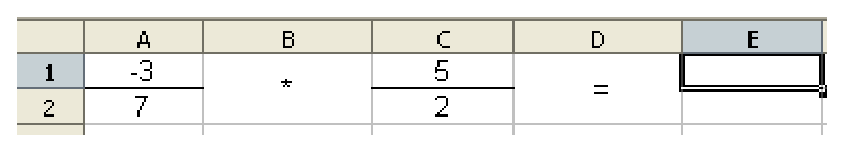
\includegraphics[width=.6\linewidth]{tableur1}
    \end{center}
    
    \begin{itemize}
        \item Recopiez les cellules ci-dessus ;
        \item Dans la cellule E1, tapez « \texttt{=A1*C1} » ;
        \item Dans la cellule E2, tapez « \texttt{=A2*C2} » ;
        \item Utilisez cette feuille de calcul pour vérifier le résultat du calcul B (question a.). Que remarquez-vous ?
    \end{itemize}
    
    \item Sur le même fichier, vous allez maintenant construire un outil permettant de calculer la somme de deux fractions.
    
    \begin{center}
        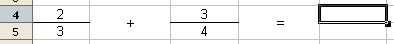
\includegraphics[width=.6\linewidth]{tableur2}
    \end{center}
    
    Recopiez les cellules ci-dessus ;
    Que faut-il taper comme formules dans les cellules E4 et E5 ?
    Utilisez cette feuille de calcul pour vérifier le résultat du calcul D (question a.). Que remarquez-vous ?
    \item Procédez de la même façon pour construire sur le même fichier quatre outils permettant :
    \begin{itemize}
        \item de calculer le produit de trois fractions ;
        \item de calculer la différence de deux fractions ;
        \item de calculer la somme de trois fractions ;
        \item de calculer le quotient de deux fractions.
    \end{itemize}
    \item Construisez un nouvel outil permettant de calculer la somme de deux fractions en faisant apparaître les étapes intermédiaires.
    \item Refaites tous les calculs avec le fichier tableur qui se trouve en complément. Quelle est la nouveauté apportée par ce fichier par rapport au vôtre ?
    \item Dans quels cas, les deux fichiers donnent-ils des résultats identiques ?
\end{enumerate}
\end{TP}

\recreation % avec R majuscule pour saut de page
%\begin{enigme}[Étourdi !]
Un abreuvoir est alimenté par deux robinets. Lorsque le robinet d'évacuation est fermé, le premier robinet seul le remplit en 4 heures. Le deuxième robinet seul le remplit en 3 heures.

\vspace{.5em}

Lorsque l'abreuvoir est plein, le robinet d'évacuation le vide en 2 heures.

\vspace{.5em}

Alors que l'abreuvoir est vide, l'éleveur ouvre les deux robinets pour le remplir,
mais oublie de fermer le robinet d'évacuation !

\vspace{.5em}

L'abreuvoir va-t-il quand même se remplir ?

Si oui, en combien de temps ?
\end{enigme}





\themaG
\chapter{Angles}\label{ChAngles}

\vspace{5cm}
\begin{acquis}
\begin{itemize}
\item Savoir repérer les angles formés par deux parallèles et une sécante (angles alternes-internes, angles alternes-externes, angles correspondants).
\item Savoir calculer des mesures d’angles en utilisant plusieurs propriétés (somme des angles d'un triangle, angles formés par deux parallèles et une sécante…).
\columnbreak
\item Savoir utiliser les propriétés des angles pour prouver que des droites sont parallèles ou perpendiculaires.
\item Savoir résoudre des problèmes en utilisant les angles.
\end{itemize}
\end{acquis}


\activites  
\begin{activite}[Les deux font la paire]



\begin{tabularx}{\linewidth}{XXXX}
\multicolumn{1}{c}{Figure 1} &
\multicolumn{1}{c}{Figure 2} &
\multicolumn{1}{c}{Figure 3} &
\multicolumn{1}{c}{Figure 4} \\
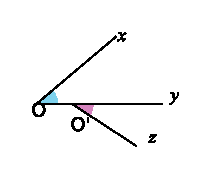
\includegraphics[width=.85\linewidth]{acti1} &

\includegraphics[width=.85\linewidth]{acti2} &
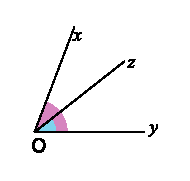
\includegraphics[width=.85\linewidth]{acti3} &
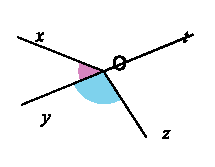
\includegraphics[width=.85\linewidth]{acti4} \\ 
\end{tabularx}

\begin{enumerate}
\item Dans les figures 2 et 4, les angles bleu et rose sont dits \textbf{adjacents}. Ce n'est pas le cas pour les autres figures. À partir de tes observations, essaie d'expliquer à quelles conditions deux angles sont adjacents. 
\item Deux angles adjacents ont-ils nécessairement la même mesure ? Justifie ta réponse.

\vspace{1em}

\begin{tabularx}{\linewidth}{XXXX}
\multicolumn{1}{c}{Figure 5} &
\multicolumn{1}{c}{Figure 6} &
\multicolumn{1}{c}{Figure 7} &
\multicolumn{1}{c}{Figure 8} \\
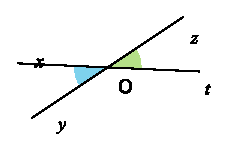
\includegraphics[width=.85\linewidth]{acti5} &

\includegraphics[width=.85\linewidth]{acti6} &
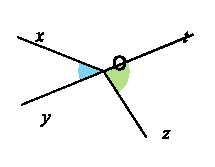
\includegraphics[width=.85\linewidth]{acti7} &
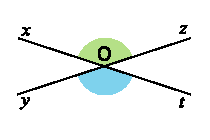
\includegraphics[width=.85\linewidth]{acti8} \\ 
\end{tabularx}

\item Dans les figures 5 et 8, les angles bleu et vert sont dits \textbf{opposés par le sommet}. Ce n'est pas le cas pour les autres figures. À partir de tes observations, essaie d'expliquer à quelles conditions deux angles sont opposés par le sommet.
\item Deux angles opposés par le sommet ont-ils nécessairement la même mesure ? Justifie ta réponse en utilisant une propriété sur deux angles symétriques par rapport à un point.
\end{enumerate}
\end{activite}


\begin{activite}[De jolies sommes !]
\begin{enumerate} \item Trace un triangle $ABC$ rectangle en $A$ puis mesure les angles $\widehat{ABC}$ et $\widehat{BCA}$.
\item Marie affirme que tous les élèves de la classe ne trouveront pas nécessairement les mêmes mesures mais qu'il y a quand même une relation entre ces deux mesures. Quelle est-elle ? Justifie ta réponse.

\vspace{1em}

On dit que deux angles sont \textbf{complémentaires} lorsque la somme de leurs mesures est égale à 90°. 
\item Les angles $\widehat{ABC}$ et $\widehat{BCA}$ sont-ils complémentaires ?
\item  Construis deux angles complémentaires \textbf{et} adjacents dont l'un mesure 64°.
\item Ahmed a mesuré l'angle $\widehat{xOz}$ ci-dessous et a trouvé 110°.

\begin{center}
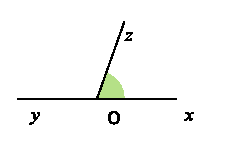
\includegraphics[width=.25\linewidth]{acti9}
\end{center}

Sa voisine lui dit que ce n'est pas possible et qu'à partir de l'erreur d'Ahmed elle pense connaître la bonne mesure. Quelle est cette mesure ? Comment a-t-elle pu la trouver ?

\vspace{1em}

On dit que deux angles sont \textbf{supplémentaires} lorsque la somme de leurs mesures est égale à 180°. 
\item Les angles $\widehat{xOz}$ et $\widehat{zOy}$ sont-ils supplémentaires ?
\item Construis deux angles supplémentaires \textbf{et} non adjacents dont l'un mesure 52°.
\end{enumerate}
\end{activite}


\begin{activite}[Avec des angles correspondants égaux...]
\begin{enumerate}
\item Observe la figure ci-dessous puis reproduis-la en choisissant la même mesure pour les angles $\widehat{ERF}$ et $\widehat{ESH}$.

\begin{center}
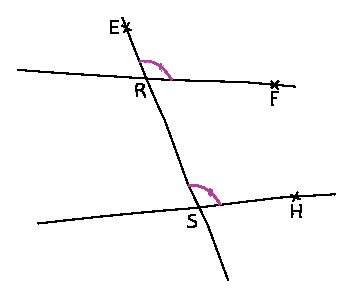
\includegraphics[width=.25\linewidth]{acti10}
\end{center}

\item\label{AactiquestionAngles} Comment peux-tu qualifier les angles $\widehat{ERF}$ et $\widehat{ESH}$ ? 
\item\label{AactiquestionDroites} Sur ta figure, quelle est la position relative des droites $(RF)$ et $(SH)$ ?
\item\label{AactiquestionPhrase} À l'aide des questions \ref{AactiquestionAngles} et \ref{AactiquestionDroites}, recopie puis complète la phrase : \textsl{« Si deux angles correspondants sont ... alors les deux droites coupées par la sécante sont ... . »}.
\item Écris une propriété identique à celle de la question \ref{AactiquestionPhrase} pour les angles alternes-internes.
\end{enumerate}
\end{activite}

\cours

\section{Caractériser deux angles ayant un sommet commun}

\begin{aconnaitre}
\textbf{Deux angles adjacents} sont deux angles qui ont un sommet commun, un côté commun et qui sont situés de part et d'autre de ce côté commun.

\vspace{.5em}

\textbf{Deux angles opposés par le sommet} sont deux angles qui ont un sommet commun et qui ont leurs côtés dans le prolongement l'un de l'autre.
\end{aconnaitre}

\begin{exemple*1}

Sur la figure ci-dessous, que peux-tu dire des angles $\widehat{AOB}$ et $\widehat{BOC}$ ?

\begin{center}
    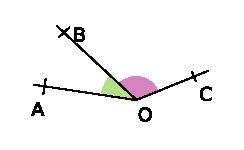
\includegraphics[width=.25\linewidth]{cours1}
\end{center}

\correction
Les angles $\widehat{AOB}$ et $\widehat{BOC}$ ont comme sommet commun le point $O$, comme côté commun la demi-droite $[OB)$ et sont placés de part et d'autre de $[OB)$ : ils sont donc adjacents.
\end{exemple*1}


\begin{exemple*1}
Sur la figure ci-dessous, que peux-tu dire des angles $\widehat{AOB}$ et $\widehat{DOE}$ ?

\begin{center}
    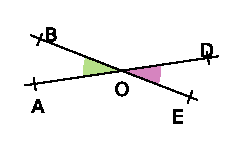
\includegraphics[width=.25\linewidth]{cours2}
\end{center}

\correction
Les angles $\widehat{AOB}$ et $\widehat{DOE}$ ont comme sommet commun le point $O$ et des côtés dans le prolongement l'un de l'autre ($A$, $O$, $D$ et $B$, $O$, $E$ sont alignés) : ils sont donc opposés par le sommet.
\end{exemple*1}

\vspace{1em}

Exercices « À toi de jouer »

Sur la figure ci-dessous, nomme trois paires d'angles adjacents.

\begin{center}
    
\includegraphics[width=.2\linewidth]{cours3}
\end{center}

Que dire des angles $\widehat{VST}$ et $\widehat{ESR}$ pour un parallélogramme $VERT$ de centre $S$ ?


\begin{aconnaitre}
Si deux angles sont opposés par le sommet \textbf{alors ils ont la même mesure.}
\end{aconnaitre}



\section{Angles complémentaires et supplémentaires}

\begin{aconnaitre}
\textbf{Deux angles complémentaires} sont deux angles dont la somme des mesures est égale à 90°.

\vspace{.5em}

\textbf{Deux angles supplémentaires} sont deux angles dont la somme des mesures est égale à 180°.
\end{aconnaitre}

\begin{exemple*1}
Sur la figure ci-dessous, que peux-tu dire des angles $\widehat{AOB}$ et $\widehat{BOC}$ ?

\begin{center}
    
\includegraphics[width=.25\linewidth]{cours4}
\end{center}

\correction
Les angles $\widehat{AOB}$ et $\widehat{BOC}$ forment un angle droit : la somme des mesures de ces angles vaut 90°. Ce sont donc des angles complémentaires.
\end{exemple*1}

\begin{remarque}
Deux angles complémentaires et adjacents forment un angle droit. On peut donc en déduire que des droites sont perpendiculaires.
\end{remarque}


\begin{exemple*1}
Sur la figure ci-dessous, que peux-tu dire des angles $\widehat{AOB}$ et $\widehat{FED}$ ?

\begin{center}
    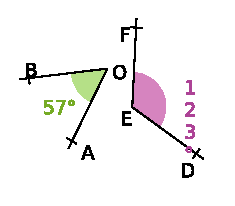
\includegraphics[width=.25\linewidth]{cours5}
\end{center}

\correction
$\widehat{AOB}+\widehat{FED}=57^\circ+123^\circ=180^\circ$ donc les angles $\widehat{AOB}$ et $\widehat{FED}$ sont supplémentaires.
\end{exemple*1}

\begin{remarque}
Deux angles supplémentaires et adjacents forment un angle plat. On peut donc en déduire que des points sont alignés.
\end{remarque}

\begin{remarque}
Deux angles complémentaires ou supplémentaires ne sont pas forcément adjacents.
\end{remarque}

\vspace{1em}

Exercices « À toi de jouer »

Les angles ci-dessous sont-ils complémentaires ?

\begin{center}
    
\includegraphics[width=.2\linewidth]{cours6}
\end{center}

Donne le complémentaire d'un angle de 27°.

Que peux-tu dire des angles aigus d'un triangle rectangle ? Justifie ta réponse.


Les angles ci-dessous sont-ils supplémentaires ?
\begin{center}
    
\includegraphics[width=.2\linewidth]{cours7}
\end{center}


Les points A, O et B sont-ils alignés ?
\begin{center}
    
\includegraphics[width=.2\linewidth]{cours8}
\end{center}







\section{Caractériser deux angles définis par deux droites et une sécante}


\begin{aconnaitre}
\begin{minipage}{.3\linewidth}
\centering

\includegraphics[width=.65\linewidth]{cours9}
\end{minipage}\hfill%
\begin{minipage}{.67\linewidth}
Les angles verts sont \textbf{alternes-internes}.

Ils sont déterminés par les droites $(d)$, $(d')$ et la sécante $(d_1)$.

Les angles roses sont \textbf{correspondants.}

Ils sont déterminés par les droites $(d)$, $(d')$ et la sécante $(d_2)$.
\end{minipage}
\end{aconnaitre}

\begin{exemple*1}
À l'aide de la figure, nomme des angles alternes-internes et des correspondants.

\begin{center}
    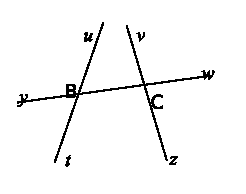
\includegraphics[width=.25\linewidth]{cours10}
\end{center}

\correction
Les droites $(ut)$, $(vz)$ et la sécante $(yw)$ forment :
\begin{itemize}
    \item deux paires d'angles alternes-internes qui sont : $\widehat{uBw}$ et $\widehat{yCz}$, $\widehat{vCy}$ et $\widehat{tBw}$.
    \item quatre paires d'angles correspondants qui sont : $\widehat{yBu}$ et $\widehat{vCy}$, $\widehat{yBt}$ et $\widehat{yCz}$, $\widehat{uBw}$ et $\widehat{vCw}$, $\widehat{tBw}$ et $\widehat{zCw}$.
\end{itemize}
\end{exemple*1}

\vspace{1em}

Exercices « À toi de jouer »

Sur la figure ci-dessous, les angles $\widehat{yOx'}$ et $\widehat{xEz'}$ sont-ils alternes-internes ? Justifie.

\begin{center}
    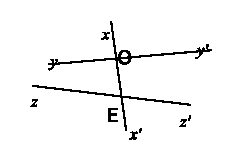
\includegraphics[width=.2\linewidth]{cours11}
\end{center}

Sur la figure  ci-dessous, nomme deux paires d'angles alternes-internes et quatre paires d'angles correspondants.

\begin{center}
    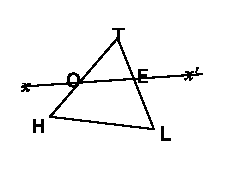
\includegraphics[width=.2\linewidth]{cours12}
\end{center}

\begin{aconnaitre}
Si deux angles alternes-internes sont déterminés par des droites parallèles \textbf{alors ils ont la même mesure.}

\vspace{.5em}

Si deux angles correspondants sont déterminés par des droites parallèles \textbf{alors ils ont la même mesure}.
\end{aconnaitre}

\begin{exemple*1}
Les droites $(vt)$ et $(uy)$ sont parallèles. Calcule la mesure des angles $\widehat{zEy}$ et $\widehat{vGw}$.

\begin{center}
    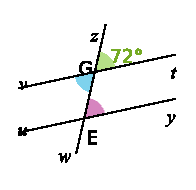
\includegraphics[width=.25\linewidth]{cours13}
\end{center}

\correction
Les angles correspondants $\widehat{zGt}$ et $\widehat{zEy}$ sont déterminés par les droites $(vt)$ et $(uy)$ qui sont parallèles. Ils sont donc de la même mesure. L'angle $\widehat{zEy}$ mesure donc 72°.

\vspace{.5em}

Les angles $\widehat{zGt}$ et $\widehat{vGw}$ sont opposés par le sommet. Ils sont donc de la même mesure. L'angle $\widehat{vGw}$ mesure donc 72°.
\end{exemple*1}

\vspace{1em}

Exercice « À toi de jouer »

Sur la figure ci-contre, les droites $(zz')$ et $(uu')$ sont parallèles. Calcule la mesure de l'angle $\widehat{x'Rz'}$ puis celle de l'angle $\widehat{uEx}$.

\begin{center}
    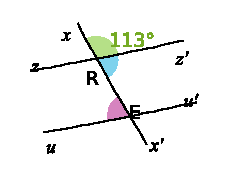
\includegraphics[width=.3\linewidth]{cours14}
\end{center}


\begin{aconnaitre}
Si deux angles alternes-internes sont de même mesure \textbf{alors les deux droites coupées par la sécante sont parallèles.}

\vspace{.5em}

Si deux angles correspondants sont de même mesure \textbf{alors les deux droites coupées par la sécante sont parallèles.}
\end{aconnaitre}


\begin{exemple*1}
Les droites $(yy')$ et $(zz')$ sont-elles parallèles ? Les droites $(xx')$ et $(uu')$ sont-elles parallèles ?

\begin{center}
    
\includegraphics[width=.3\linewidth]{cours15}
\end{center}

\correction
Les angles $\widehat{x'Ay'}$ et $\widehat{xBz}$ déterminés par les droites $(yy')$, $(zz')$ et la sécante $(xx')$ sont alternes-internes. Les angles $\widehat{x'Ay'}$ et $\widehat{xBz}$ ont la même mesure.

Donc les droites $(yy')$ et $(zz')$ sont parallèles.

\vspace{.5em}

Les angles $\widehat{x'Ay'}$ et $\widehat{u'Dy'}$ déterminés par les droites $(xx')$, $(uu')$ et la sécante $(yy')$ sont correspondants. Si les droites $(xx')$ et $(uu')$ étaient parallèles alors les angles $\widehat{x'Ay'}$ et $\widehat{u'Dy'}$ seraient de la même mesure, ce qui n'est pas le cas.

Donc les droites $(xx')$ et $(uu')$ ne sont pas parallèles.
\end{exemple*1}

\vspace{1em}

Exercice « À toi de jouer »

Dans chacun des cas ci-dessous, indique si les droites $(AB)$ et $(OT)$ sont parallèles. Justifie ta réponse.

\begin{center}
\begin{minipage}{.48\linewidth}
\centering
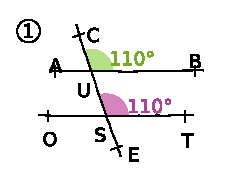
\includegraphics[width=.45\linewidth]{cours16}
\end{minipage}\hfill%
\begin{minipage}{.48\linewidth}
\centering
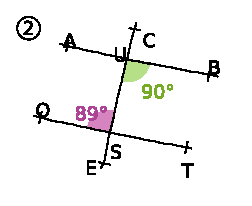
\includegraphics[width=.45\linewidth]{cours17}
\end{minipage}
\end{center}


\exercicesbase
\begin{colonne*exercice}
\serie{Propriétés des triangles}


\begin{exercice}[Reconnaître]
Donne, en justifiant, la nature de chacun des triangles s'il est particulier.
\begin{colenumerate}{4}
\item 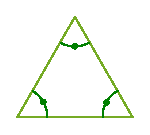
\includegraphics[width=.8\linewidth]{exoEnt1}
\item 
\includegraphics[width=.8\linewidth]{exoEnt2}
\item 
\includegraphics[width=.8\linewidth]{exoEnt3}
\item 
\includegraphics[width=.8\linewidth]{exoEnt4}
\end{colenumerate}
\end{exercice}



\begin{exercice}
Dans chaque cas, effectue un croquis puis construis la figure.
\begin{colenumerate}{1}
\item Trace un triangle $FIN$ rectangle en $F$ tel que $FI$ = 5 cm et $NF$ = 6 cm.
\item Trace un triangle $TRS$ rectangle en $S$ tel que $TS$ = 72 mm et $SR$ = 85 mm.
\item Construis un triangle $MNO$ équilatéral de côté 5 cm.
\item Construis un triangle isocèle $STU$ isocèle en $S$ tel que $ST$ = 58 mm et $TU$ = 32 mm.
\item Construis un triangle $ABC$ tel que $AB$ = 6 cm ; $BC$ = 5,2 cm et $CA$ = 42 mm.
\end{colenumerate}
\end{exercice}



\begin{exercice}[Médiatrices dans un triangle]
\begin{enumerate}
\item Construis un triangle $ABC$ tel que $AB$ = 5,7 cm, $AC$ = 5,3 cm et $BC$ = 7 cm.
\item Construis les médiatrices des segments $[AB]$ et $[CB]$. Note $O$ leur point d'intersection.
\item Construis la médiatrice du segment $[AC]$. Que constates‑tu ?
\item Trace le cercle de centre $O$ passant par $A$. Comment s'appelle ce cercle ?
\end{enumerate}
\end{exercice}



\begin{exercice}[Bissectrice dans un triangle]
\begin{enumerate}
\item Trace un triangle $UST$ tel que $UT$ = 6 cm ; $US$ = 10 cm et $ST$ = 14 cm.
\item Construis les bissectrices des angles $\widehat{UST}$, $\widehat{UTS}$ et $\widehat{TUS}$.

Que constates‑tu ?
\end{enumerate}
\end{exercice} 




\begin{exercice}
Dans les 6 cas suivants, détermine si la droite $d$ est :
\begin{enumerate}
\item une hauteur ;
\item une médiatrice ;
\item une bissectrice ;
\item une médiane.
\end{enumerate}

\begin{colenumerate}{3}
\item 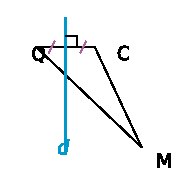
\includegraphics[width=.8\linewidth]{exoEnt5}
\item 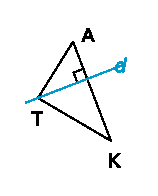
\includegraphics[width=.8\linewidth]{exoEnt6}
\item 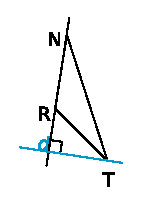
\includegraphics[width=.8\linewidth]{exoEnt7}
\item 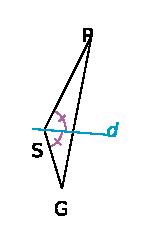
\includegraphics[width=.8\linewidth]{exoEnt8}
\item 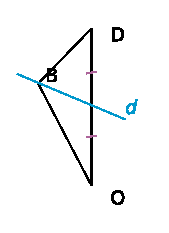
\includegraphics[width=.8\linewidth]{exoEnt9} 
\item 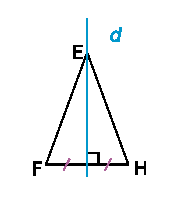
\includegraphics[width=.8\linewidth]{exoEnt10}
\end{colenumerate}
\end{exercice}




\begin{exercice}[Vocabulaire]
\begin{enumerate}
\item Construis un triangle $BOA$ tel que $BO$ = 5 cm, $OA$ = 7 cm et $AB$ = 8 cm. Trace la droite $d_1$ perpendiculaire à $[BO]$ et passant par $A$.
\item Trace la droite $d_2$ perpendiculaire au segment $[OA]$ et passant par son milieu.
\item Trace la droite $d_3$ qui coupe l'angle $\widehat{OBA}$ en deux angles égaux.
\item Trace la droite $d_4$ qui passe par $O$ et par le milieu de $[BA]$.
\item Détermine quelle(s) droite(s) représente(nt) la hauteur du triangle.
\item Détermine quelle(s) droite(s) représente(nt) une médiatrice.
\item Détermine quelle(s) droite(s) représente(nt) une bissectrice.
\item Détermine quelle(s) droite(s) représente(nt) une médiane.
\end{enumerate}
\end{exercice}




\begin{exercice}[Hauteurs d'un triangle]
Construis un triangle $BON$ tel que $BO$ = 68 mm, $BN$ = 62 mm et $NO$ = 45 mm.

Trace :
\begin{itemize}
\item en noir, la perpendiculaire à $(BN)$ passant par $O$ ;
\item en rouge, la perpendiculaire à $(NO)$ passant par $B$ ;
\item en vert, la perpendiculaire à $(BO)$ passant par $N$. Que remarques‑tu ?
\end{itemize}
\end{exercice}


\begin{exercice}[Hauteur (« relative à » ou « issue de »)]
\begin{enumerate}
\item Construis un triangle $AVE$ quelconque puis trace :
    \begin{itemize}
    \item en bleu, la hauteur issue du sommet $E$ ;
    \item en noir, la hauteur issue du sommet $A$ ;
    \item en rouge, la hauteur relative à $[AE]$.
    \end{itemize}
\item Observe ces trois hauteurs. Quelle remarque peux-tu faire ?
\end{enumerate}
\end{exercice}



\begin{exercice}[À l'intérieur ou pas ?]
\begin{enumerate}
\item Construis un triangle $DER$ ayant tous ses angles aigus. Trace les hauteurs de ce triangle.
\item Construis un triangle $NRV$ tel que $\widehat{NRV}$ soit un angle obtus. Trace les hauteurs de ce triangle.
\item Construis un triangle $GHT$ rectangle en $T$. Trace les hauteurs de ce triangle.
\item Observe les trois figures. Quelles remarques peux-tu faire ?
\end{enumerate}
\end{exercice}



\begin{exercice}[Vocabulaire] 
\begin{enumerate}
\item Construis un triangle $OA$. Trace la droite $(d_1)$ perpendiculaire à $[BO]$ et passant par $A$.
\item Trace la droite $(d_2)$ perpendiculaire au segment $[OA]$ et passant par son milieu.
\item Trace la droite $(d_3)$ qui coupe l'angle $\widehat{BOA}$ en deux angles égaux.
\item Trace la droite $(d_4)$ qui passe par $O$ et par le milieu de $[BA]$.
\item Reformule les questions précédentes en utilisant les mots : médiatrice, bissectrice, médiane et hauteur.
\end{enumerate}
\end{exercice}



\begin{exercice}[Cercles circonscrits]
Dans chaque cas, construis le triangle $LYS$ puis son cercle circonscrit.
\begin{enumerate}
\item $LS$ = 8 cm, $\widehat{YLS}$ = 65° et $\widehat{YSL}$ = 45°.
\item $LS$ = 4 cm, $LY$ = 5 cm et $\widehat{YLS}$ = 103°.
\item $LYS$ est isocèle en $L$ tel que $LY$ = 8 cm et $YS$ = 5,5 cm.
\item $LYS$ est un triangle équilatéral de côté 6 cm.
\end{enumerate}
\end{exercice}




\begin{exercice}[Sois malin !]
\begin{enumerate}
\item Construis un triangle $MEC$ tel que son cercle circonscrit ait un rayon de 5 cm.
\item Construis un triangle $RNB$ isocèle en $B$ avec $BN$ = 4 cm tel que son cercle circonscrit ait un rayon de 5 cm.
\end{enumerate}
\end{exercice}



\begin{exercice}[Cercle inscrit]
Dans chaque cas, construis le triangle $ABC$ puis son cercle inscrit.
\begin{enumerate}
\item $AC$ = 8 cm, $\widehat{BAC}$ = 60° et $\widehat{ACB}$ = 50°.
\item $AC$ = 10 cm, $AB$ = 8 cm et $\widehat{BAC}$ = 45°.
\item $ABC$ est isocèle en $A$ tel que $AB$ = 9 cm et $BC$ = 6 cm.
\item $ABC$ est un triangle équilatéral de côté 7,5 cm.
\end{enumerate}
\end{exercice}



\serie{Utiliser le vocabulaire associé aux angles}






\begin{exercice}
$\hat{a}$ et $\hat{b}$ sont deux angles complémentaires.

Calcule la mesure de $\hat{b}$ si :

$\hat{a}$ = 45°,\hfill%
$\hat{a}$ = 37°,\hfill%
$\hat{a}$ = 2°,\hfill%
$\hat{a}$ = 88,3°.  
\end{exercice}



\begin{exercice}
$\hat{x}$ et $\hat{y}$ sont deux angles supplémentaires.

Calcule la mesure de $\hat{y}$ si :

$\hat{x}$= 103°,\hfill%
$\hat{x}$= 95°,\hfill%
$\hat{x}$= 56°,\hfill%
$\hat{x}$= 0,3°.
\end{exercice}




\begin{exercice}
Indique si les angles proposés sont adjacents, complémentaires ou bien encore supplémentaires. Justifie tes réponses. 

\begin{center}
    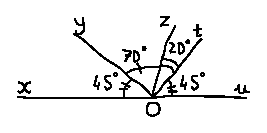
\includegraphics[width=.8\linewidth]{exoEnt11}
\end{center}

\begin{enumerate}
\item $\widehat{yOz}$ et $\widehat{zOt}$ ;
\item $\widehat{xOy}$ et $\widehat{yOu}$ ;
\item $\widehat{xOy}$ et $\widehat{tOu}$ ;
\item $\widehat{yOu}$ et $\widehat{tOu}$ ;
\item $\widehat{xOz}$ et $\widehat{zOt}$ ;
\item $\widehat{xOt}$ et $\widehat{uOt}$.
\end{enumerate}
\end{exercice}


\columnbreak
\begin{exercice}[Les deux font la paire]
Nomme, en justifiant, deux angles de la figure, codés ou non :
\begin{enumerate}
\item complémentaires et adjacents ;
\item complémentaires et non adjacents ;
\item supplémentaires et adjacents ;
\item supplémentaires et non adjacents ;
\item opposés par le sommet.
\end{enumerate}

\begin{center}
    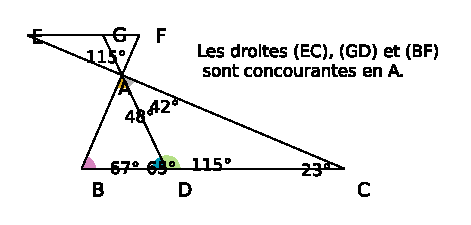
\includegraphics[width=\linewidth]{exoEnt12}
\end{center}

\end{exercice}




\begin{exercice}[Les angles inconnus]
\begin{enumerate}
\item Trouve la mesure de deux angles complémentaires, sachant que l'un d'eux est 8 fois plus grand que l'autre.
\item Trouve la mesure de deux angles supplémentaires, sachant que l'un d'eux est 9 fois plus petit que l'autre.
\end{enumerate}
\end{exercice}



\begin{exercice}[Des angles dynamiques...]
\begin{enumerate}
\item À l'aide du logiciel \emph{TracenPoche}, construis deux angles complémentaires et adjacents.
\item Propose une façon de procéder pour que ces angles restent adjacents, complémentaires et égaux à 45°, même quand on bouge les points.
\end{enumerate}
\end{exercice}



\begin{exercice}
Que peut-on dire des angles :

\begin{minipage}{.3\linewidth}
\begin{enumerate}
\item 1 et 3 ?
\item 1 et 5 ?
\item 3 et 5 ?
\item 1 et 4 ?
\item 4 et 6 ?
\item 3 et 7 ?
\end{enumerate}
\end{minipage}\hfill%
\begin{minipage}{.67\linewidth}
\centering
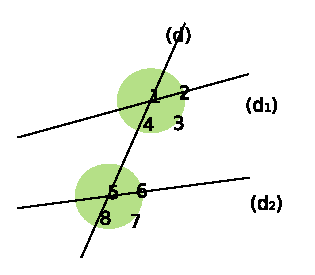
\includegraphics[width=\linewidth]{exoEnt13}
\end{minipage}
\end{exercice}




\begin{exercice}
Nomme deux angles de la figure et précise le nom de la sécante correspondante :
\begin{enumerate}
\item alternes-internes avec l'angle \no 3 ;
\item correspondants avec l'angle \no 10 ;
\item alternes-internes avec l'angle \no 13 ;
\item correspondants avec l'angle \no 7.
\end{enumerate}

\begin{center}
    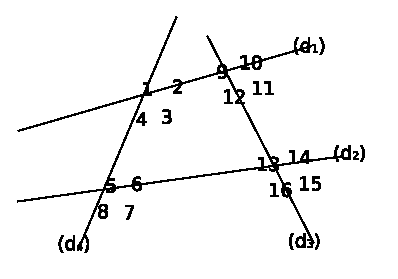
\includegraphics[width=.8\linewidth]{exoEnt14}
\end{center}

\end{exercice}



\begin{exercice}[Recherche de mesures d'angles]
\begin{enumerate}
\item Nomme deux paires d'angles de la figure :
    \begin{itemize}
    \item alternes-internes aigus ;
    \item alternes-internes de même mesure ;
    \item correspondants aigus ;
    \item supplémentaires et non adjacents.
    \end{itemize}
    
\begin{center}
    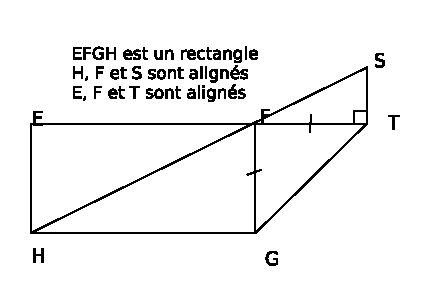
\includegraphics[width=.9\linewidth]{exoEnt15}
\end{center}

\item Sachant de plus que $\widehat{EFH}$ = 27°, calcule la mesure de l'angle $\widehat{SFT}$ puis celle de $\widehat{SFG}$.
\end{enumerate}
\end{exercice}

\columnbreak
\serie{Caractériser des droites parallèles par les angles}



\begin{exercice}
Dans chaque cas, dire si les droites $(d_1)$ et $(d_2)$ sont ou non parallèles et pourquoi.
\begin{center}
    \includegraphics[width=.8\linewidth]{exoEnt16}
\end{center}
\end{exercice} 



\begin{exercice}[Le coup des équerres !]
Arnaud a placé ses deux équerres identiques sur la droite $(d)$ comme l'illustre le schéma ci-dessous.

\begin{center}
    \includegraphics[width=.8\linewidth]{exoEnt17}
\end{center}

\begin{enumerate}
\item Il affirme que, de cette façon, il peut tracer des droites parallèles. Est-ce vrai et pourquoi ?
\item Quelles seraient les autres façons de positionner les équerres pour obtenir le même résultat ?
\end{enumerate}
\end{exercice} 



\begin{exercice}[Angles et droites parallèles]

\begin{center}
    \includegraphics[width=.8\linewidth]{exoEnt18}
\end{center}

\begin{enumerate}
\item Calcule la mesure de l'angle $\widehat{uBr}$.
\item Les droites $(xy)$ et $(sr)$ sont-elles parallèles ? Justifie ta réponse.
\end{enumerate}
\end{exercice}



\columnbreak
\serie{Calculer des angles formés par des\\ droites parallèles}





\begin{exercice}[Parallèles ?]
Sur la figure ci-dessous, les angles $\widehat{BAE}$ et $\widehat{FEO}$ sont égaux à 58°.

\begin{center}
    \includegraphics[width=.7\linewidth]{exoEnt19}
\end{center}

\begin{enumerate}
\item Que peux-tu dire des droites $(EF)$ et $(AB)$ ? Justifie ta réponse.
\item On sait de plus que la mesure de l'angle $\widehat{FBA}$ est 45°. Déduis-en la mesure de l'angle $\widehat{OFE}$. Justifie ta réponse.
\end{enumerate}
\end{exercice}


\begin{exercice}[Droites parallèles]

\begin{center}
    \includegraphics[width=.7\linewidth]{exoEnt20}
\end{center}

Sur la figure ci-dessus, les droites $(xy)$ et $(zt)$ sont parallèles. L'angle $\widehat{xMu}$ vaut 125°.
\begin{enumerate}
\item Donne la mesure de l'angle $\widehat{vMy}$. Justifie ta réponse.
\item Donne d'autres angles dont la mesure est de 125°. Justifie ta réponse.
\end{enumerate}
\end{exercice}

\newpage
\begin{exercice}[Angles supplémentaires]
                        
\begin{center}
    \includegraphics[width=\linewidth]{exoEnt21}
\end{center}
                                 
\begin{enumerate}
\item Justifie que les angles $\widehat{BAC}$ et $\widehat{BDC}$ sont de même mesure.
\item Que dire des angles $\widehat{BDC}$ et $\widehat{BDE}$ ? Pourquoi ? Justifie alors que les deux angles marqués sont supplémentaires.
\end{enumerate}
\end{exercice}

\columnbreak
\begin{exercice}[Zigzag]

\begin{center}
    \includegraphics[width=.8\linewidth]{exoEnt22}
\end{center}

Sur la figure ci-dessus :
\begin{itemize}
    \item les droites $(AB)$, $(CD)$ et $(EF)$ sont parallèles ;
    \item $R$ est un point de la droite $(AB)$, $S$ est un point de la droite $(CD)$ et $T$ est un point de la droite $(EF)$ tels que : $\widehat{BRS}$ = 20° et $\widehat{RST}$ = 57°.
\end{itemize}

Calcule la mesure de l'angle $\widehat{STF}$.
\end{exercice}


\begin{exercice}
Construis à l'aide de \emph{TracenPoche} un quadrilatère $EFGH$ ayant deux angles droits, en $E$ et en $G$.
\begin{enumerate}
\item Affiche la mesure des angles $\widehat{EFG}$ et $\widehat{EHG}$. Que remarques-tu ?
\item Trace le segment $[FH]$. En raisonnant dans les triangles $EFH$ et $FHG$, démontre que $\widehat{EFG}$ et $\widehat{EHG}$ sont supplémentaires.
\end{enumerate}
\end{exercice}

\end{colonne*exercice}


\exercicesappr
\begin{colonne*exercice}
\begin{exercice}
Dans chaque cas, précise si les droites $(d_1)$ et $(d_2)$ sont ou non parallèles et pourquoi.

\begin{center}
    \includegraphics[width=\linewidth]{exoApp1}
\end{center}

\end{exercice}



\begin{exercice}[Triangle isocèle]

\begin{center}
    \includegraphics[width=.8\linewidth]{exoApp2}
\end{center}

La figure ci-dessus est telle que :
\begin{itemize}
    \item $B$, $A$ et $D$ sont des points alignés ;
    \item $\widehat{BAC}$ et $\widehat{ACD}$ sont supplémentaires ;
    \item $\widehat{BAC}$= 110°.
\end{itemize}

\begin{enumerate}
\item Montre, en justifiant, que les angles $\widehat{DAC}$ et $\widehat{ACD}$ sont égaux à 70°.
\item Montre alors que le triangle $ADC$ est isocèle.
\item De plus, l'angle $\widehat{ACB}$ mesure 50°. Montre, en justifiant, que les angles $\widehat{BCA}$ et $\widehat{ADC}$ sont complémentaires.
\item Trouve, en justifiant, deux autres paires d'angles complémentaires.
\end{enumerate}
\end{exercice}




\begin{exercice}[Parallèles ou non ?]

\begin{center}
    \includegraphics[width=.8\linewidth]{exoApp3}
\end{center}

La figure ci-dessus est tracée à main levée.

\begin{enumerate}
\item Calcule la mesure de l'angle $\widehat{LON}$.
\item Déduis-en la mesure de l'angle $\widehat{ONL}$.
\item Détermine alors si les droites $(LN)$ et $(MP)$ sont parallèles.
\item Sachant que les segments $[LN]$ et $[MP]$ sont de même longueur, détermine la nature du quadrilatère $LNPM$.
\end{enumerate}
\end{exercice}




\begin{exercice}[Un isocèle de plus]

\begin{center}
    \includegraphics[width=.6\linewidth]{exoApp4}
\end{center}

La figure ci-dessus est telle que :
\begin{itemize}
    \item les droites $(RO)$ et $(SN)$ sont sécantes en $T$ ;
    \item le triangle $RST$ est isocèle en $R$ ;
    \item les droites $(RS)$ et $(NO)$ sont parallèles.
\end{itemize}

Montre que le triangle $TNO$ est isocèle.
\end{exercice}




\begin{exercice}[Un périscope de fortune !]

\begin{enumerate}
\item Fais une recherche sur Internet concernant la loi de réflexion de la lumière.
\item Le schéma ci-dessous illustre un rayon de lumière qui se réfléchit sur un miroir avec un angle de 30°. Détermine $\hat{x}$ et $\hat{y}$. Justifie.

\begin{center}
    \includegraphics[width=.8\linewidth]{exoApp5}
\end{center}

\item Éric a construit un périscope avec une boîte de carton et deux miroirs parallèles comme l'illustre le schéma ci-dessous.

\begin{center}
    \includegraphics[width=.8\linewidth]{exoApp6}
\end{center}

\begin{itemize}
    \item Si un rayon entre horizontalement dans le périscope, en sortira-t-il horizontalement aussi ?
    
    (Tu pourras montrer que les rayons d'entrée et de sortie sont parallèles.)
    \item Ce résultat dépend-il de l'inclinaison des miroirs parallèles ?
    
    (Autrement dit, a-t-on le même résultat si l'angle formé par le rayon et le miroir est différent de 45° ?)
\end{itemize}
\end{enumerate}
\end{exercice}

\end{colonne*exercice}

\connaissances
\QCMautoevaluation{Pour chaque question, plusieurs réponses sont proposées. Déterminer celles qui sont correctes.}

\begin{QCM}

\begin{GroupeQCM}


\begin{exercice}
Parmi les couples d'angles suivants, quels sont ceux qui sont complémentaires ?
\begin{ChoixQCM}{2}
\item $\widehat{FEG}=8$° et $\widehat{HIK}=82$°
\item $\widehat{FEG}=90$° et $\widehat{HIK}=90$°
\item $\widehat{ABC}=73$° et $\widehat{STU}=107$°
\item $\widehat{FEG}=89,9$° et $\widehat{HIK}=0,1$°
\end{ChoixQCM}
\begin{corrige}
\reponseQCM{a}
\end{corrige}
\end{exercice}
\end{GroupeQCM}



\begin{EnonceCommunQCM}
Les questions \RefQCM{Aqcm1} et \RefQCM{Aqcm2} se rapportent à la figure ci-dessous.
\begin{center}
    \includegraphics[width=.25\linewidth]{qcm1}
    
    $E$, $R$ et $I$ sont alignés.
\end{center}
\end{EnonceCommunQCM}

\begin{GroupeQCM}


\begin{exercice}\label{Aqcm1}
Les angles...
\begin{ChoixQCM}{2}
\item $\widehat{ERH}$ et $\widehat{HRI}$ sont supplémentaires
\item $\widehat{FRG}$ et $\widehat{HRI}$ sont adjacents
\item $\widehat{ERG}$ et $\widehat{FRI}$ sont supplémentaires
\item $\widehat{FRG}$ et $\widehat{GRH}$ sont adjacents
\end{ChoixQCM}
\begin{corrige}
\reponseQCM{a}
\end{corrige}
\end{exercice}





\begin{exercice}\label{Aqcm2}
L'angle...
\begin{ChoixQCM}{2}
\item $\widehat{FRG}$ est le complémentaire de $\widehat{GRH}$
\item $\widehat{FRE}$ est le complémentaire de $\widehat{HRI}$
\item $\widehat{ERF}$ est le complémentaire de $\widehat{FRI}$
\item $\widehat{GRH}$ est le complémentaire de $\widehat{HRI}$
\end{ChoixQCM}
\begin{corrige}
\reponseQCM{a}
\end{corrige}
\end{exercice}
\end{GroupeQCM}
\end{QCM}

\begin{QCM}

\begin{EnonceCommunQCM}
Les questions \RefQCM{Aqcm3}, \RefQCM{Aqcm4} et \RefQCM{Aqcm5} se rapportent à la figure ci-dessous.
\begin{center}
    \includegraphics[width=.25\linewidth]{qcm2}
    
    $(AD)$ et $(FH)$ sont parallèles.
\end{center}
\end{EnonceCommunQCM}

\begin{GroupeQCM}

\begin{exercice}\label{Aqcm3}

\begin{ChoixQCM}{2}
\item $\widehat{ACH}$ et $\widehat{BCD}$ sont opposés par le sommet
\item $\widehat{CDF}$ et $\widehat{BCD}$ sont opposés par le sommet
\item $\widehat{ACH}$ et $\widehat{BCD}$ sont adjacents
\item $\widehat{BCD}$ et $\widehat{CHF}$ sont correspondants
\end{ChoixQCM}
\begin{corrige}
\reponseQCM{a}
\end{corrige}
\end{exercice}




\begin{exercice}\label{Aqcm4}

\begin{ChoixQCM}{4}
\item $\widehat{BCD}=100$°
\item $\widehat{BHF}=100$°
\item $\widehat{BCA}=100$°
\item $\widehat{DCH}=100$°
\end{ChoixQCM}
\begin{corrige}
\reponseQCM{a}
\end{corrige}
\end{exercice}




\begin{exercice}\label{Aqcm5}

\begin{ChoixQCM}{4}
\item $\widehat{CDF}=40$°
\item $\widehat{BFH}=50$°
\item $\widehat{DCH}=80$°
\item $\widehat{CDF}=100$°
\end{ChoixQCM}
\begin{corrige}
\reponseQCM{a}
\end{corrige}
\end{exercice}



\begin{exercice}
\begin{center}
    \includegraphics[width=.25\linewidth]{qcm3}
\end{center}
\begin{ChoixQCM}{4}
\item Si les angles roses sont égaux alors $(d)$ et $(d')$ sont parallèles
\item Si $(d)$ et $(d')$ sont parallèles alors les angles roses sont égaux
\item Les angles roses sont correspondants
\item Les angles roses sont alternes-internes
\end{ChoixQCM}
\begin{corrige}
\reponseQCM{a}
\end{corrige}
\end{exercice}


\begin{exercice}
Quelles sont les affirmations vraies ?
\begin{ChoixQCM}{4}
\item $\widehat{OUG}$ et $\widehat{ZKL}$ sont opposés par le sommet
\item Deux angles alternes-internes peuvent être opposés par le sommet
\item Deux angles correspondants peuvent être opposés par le sommet
\item Le supplémentaire d'un angle aigu est obtus
\end{ChoixQCM}
\begin{corrige}
\reponseQCM{a}
\end{corrige}
\end{exercice}




\begin{exercice}
\begin{center}
    \includegraphics[width=.25\linewidth]{qcm4}
    
    $(TR)$ et $(SU)$ sont parallèles et $\widehat{REA}$=60°.
\end{center}
\begin{ChoixQCM}{4}
\item $\widehat{EAS}=60$°
\item $\widehat{TEA}=120$°
\item $\widehat{EAU}=60$°
\item $\widehat{EAU}=90$°
\end{ChoixQCM}
\begin{corrige}
\reponseQCM{a}
\end{corrige}
\end{exercice}

\end{GroupeQCM}
\end{QCM}

\TravauxPratiques
\begin{TP}[Triominos avec les angles]


\textbf{1\up{ère} étape : calculer et justifier}

\begin{enumerate}
\item Voici six figures. Pour chacune d'elles, calculez, en justifiant votre calcul, l'angle marqué par un point d'interrogation. (Les droites d'une même couleur sont parallèles.)

\begin{center}
    \includegraphics[width=.6\linewidth]{tabImage}
\end{center}


\item Voici six énoncés. Pour chacun d'eux, répondez à la question en justifiant la réponse :

\begin{center}
    \includegraphics[width=.6\linewidth]{tabType}
\end{center}


\vspace{1em}\textbf{2\up{e} étape : construction des triominos}\vspace{1em}

\item \label{AtpTabType} Voici un tableau qui va vous permettre de construire le jeu de triominos. 

\begin{center}
    \includegraphics[width=.6\linewidth]{tableau}
\end{center}

Toutes les cases d'une même colonne renvoient à l'angle indiqué en ligne 1. Par exemple, les cases F2, F3... renvoient à un angle de 110°.

Pour le type \textbf{t3}, mettez aussi des exemples d'angles correspondants.

\item Dans une feuille blanche au format A4, construisez 10 triangles équilatéraux de 9 cm de côté. Utilisez une seconde feuille pour obtenir 20 triominos au total. Complétez chacun d'eux avec les énoncés ou constructions indiqués dans le tableau de la question \ref{AtpTabType}. en respectant l'ordre donné ci-dessous. Pour vous aider, voici un exemple pour le premier triomino de la série :

\hfill\includegraphics[width=.15\linewidth]{tp7} \hfill \includegraphics[width=.3\linewidth]{tp8}\hfill\phantom{.}
 
\begin{center}
    \includegraphics[width=.75\linewidth]{tp9}
    
    \includegraphics[width=.75\linewidth]{tp10}
\end{center}

\vspace{1em}\textbf{3\up{e} étape : par équipe de deux joueurs}\vspace{1em}

Retournez tous les triominos pour former la pioche. Chaque joueur en prend quatre.      

Un triomino est tiré dans la pioche pour servir de départ. Chaque joueur place à son tour un triomino. (Les côtés qui se touchent doivent correspondre à des angles égaux.)

Si le joueur ne peut pas jouer, il passe son tour \textbf{et} pioche. Le premier joueur qui n'a plus de triomino est déclaré vainqueur.

\textbf{Attention} : si un joueur se trompe en plaçant un triomino, il doit le reprendre et tirer un triomino supplémentaire dans la pioche ; c'est alors à son adversaire de jouer...
\end{enumerate}

\end{TP}

\recreation % avec R majuscule pour saut de page
\begin{enigme}[Un problème de construction]
Trace une droite $(d)$ et place un point $A$ n'appartenant pas à $(d)$.

Construis un triangle équilatéral dont un des sommets est $A$ et les deux autres sommets sont deux points de la droite $(d)$.

Propose une méthode de construction à l'aide d'un logiciel de géométrie dynamique.
\end{enigme}





\AfficheListeMethodes
\AfficheCorriges[2]
\AfficheLexique

\end{document}
